\documentclass[11pt]{article}
\usepackage[T1]{fontenc}
\usepackage[utf8]{inputenc}
\usepackage{fourier}
\usepackage[scaled=0.875]{helvet}
\renewcommand{\ttdefault}{lmtt}
\usepackage{amsmath,amssymb}
\usepackage{makeidx}
\makeindex
\usepackage{fancybox}
\usepackage[normalem]{ulem}
\usepackage{pifont}
\newcommand{\textding}[1]{\text{\ding{#1}}}
\usepackage{lscape}
\usepackage{tabularx,booktabs}
\usepackage{tabularray}%pour tableau tblr
\usepackage{scratch3}
\usepackage{textcomp}
\usepackage{enumitem}
\usepackage{multicol}
\usepackage{multirow}
\definecolor{scrmovedddd}{HTML}{3373cc}%
\newcommand{\euro}{\eurologo{}}
%Tapuscrit : Denis Vergès 
\usepackage{pst-eucl}
\usepackage{diagbox}% à mettre après pst-eucl
\usepackage{graphicx,pstricks,pst-plot,pst-grad,pst-node,pst-text,pstricks-add}
\DeclareGraphicsExtensions{.bmp,.png,.pdf,.jpg}
\usepackage{pstricks-add}
\usepackage{pgf,tikz,pgfplots}
\usetikzlibrary{patterns,calc,decorations.pathmorphing}
\newcommand{\R}{\mathbb{R}}
\newcommand{\N}{\mathbb{N}}
\newcommand{\D}{\mathbb{D}}
\newcommand{\Z}{\mathbb{Z}}
\newcommand{\Q}{\mathbb{Q}}
\newcommand{\C}{\mathbb{C}}
\usepackage[left=3.5cm, right=3.5cm, top=2.2cm, bottom=2cm]{geometry}
\setlength\headheight{13.7pt}
\newcommand{\vect}[1]{\overrightarrow{\,\mathstrut#1\,}}
\renewcommand{\theenumi}{\textbf{\arabic{enumi}}}
\renewcommand{\labelenumi}{\textbf{\theenumi.}}
\renewcommand{\theenumii}{\textbf{\alph{enumii}}}
\renewcommand{\labelenumii}{\textbf{\theenumii.}}
\def\Oij{$\left(\text{O}~;~\vect{\imath},~\vect{\jmath}\right)$}
\def\Oijk{$\left(\text{O}~;~\vect{\imath},~\vect{\jmath},~\vect{k}\right)$}
\def\Ouv{$\left(\text{O}~;~\vect{u},~\vect{v}\right)$}
\usepackage{fancyhdr}
\usepackage[french]{babel}
\usepackage[np]{numprint}
\usepackage{colortbl}
%\usetikzlibrary{backgrounds}
%\usetikzlibrary{calc,shapes.arrows,decorations.pathreplacing}

\usepackage[colorlinks=true,linkcolor=blue,citecolor=blue,urlcolor=blue]{hyperref}
\hypersetup{%
pdfauthor = {APMEP},
pdfsubject = {Brevet},
pdftitle = {Année 2023},
allbordercolors = white,
pdfstartview=FitH}
\usepackage[french]{babel}
\usepackage[np]{numprint}
\begin{document}
\setlength\parindent{0mm}
\marginpar{\rotatebox{90}{\textbf{A. P{}. M. E. P{}.}}}
\rhead{\textbf{A. P{}. M. E. P{}.}}
\lhead{\small L'intégrale 2024}

\pagestyle{fancy}
\thispagestyle{empty}
\begin{center} {\Large \textbf{\decofourleft~Brevet des collèges 2024~\decofourright\\\vspace{1cm} L'intégrale de mai 2024 à décembre 2024}}

\vspace{1cm}

Pour un accès direct cliquez sur les liens {\Large \textcolor{blue}{bleus}}
\end{center}

\phantomsection 
\label{sommaire}
\hypertarget{sommaire}{}

\begin{tabularx}{\linewidth}{>{\Large}X}

\hyperlink{AmeriqueduNord}{Amérique du Nord - 29 mai 2024}\dotfill \pageref{AmeriqueduNord} \\[7pt]
\hyperlink{Etranger}{Centres étrangers - 10 juin 2024} \dotfill \pageref{Etranger} \\[7pt]
\hyperlink{Asie}{Asie - 19 juin 2024} \dotfill \pageref{Asie} \\[7pt]
\hyperlink{Polynesie}{Polynésie - 27 juin 2024} \dotfill \pageref{Polynesie} \\[7pt]
\hyperlink{Metropole}{Métropole, La Réunion, Guadeloupe, Guyane - 1\up{er} juillet 2024} \dotfill \pageref{Metropole}\\[7pt]
\hyperlink{Martinique}{Martinique - 3 juillet 2024} \dotfill \pageref{Martinique}\\[7pt]
\hyperlink{Polynesiesep}{Polynésie 9 septembre 2024} \dotfill \pageref{Polynesiesep} \\[7pt]
\hyperlink{Metropolesep}{Métropole, La Réunion, Antilles--Guyane 19 sept. 2024} \dotfill \pageref{Metropolesep} \\
\hyperlink{AmeriqueSud}{Amérique du Sud 2 décembre 2024}  \dotfill \pageref{AmeriqueSud} \\[7pt]
\hyperlink{Caledoniedec}{Nouvelle-Calédonie décembre 2024} Contrôle continu \dotfill \pageref{Caledoniedec} 
\end{tabularx}

\vspace{1cm}

\hyperlink{Index}{À la fin index des notions abordées}

\newpage
~
\newpage
%%%%%%%%   Amérique du Nord 29  mai 2024

%\rhead{\textbf{A. P{}. M. E. P{}.}}

\phantomsection

\hypertarget{AmeriqueduNord}{}
\label{AmeriqueduNord}

\lhead{\small L'année 2024}
\rhead{\small \textbf{A. P{}. M. E. P{}.}}
\rfoot{\small Amérique du Nord }
\lfoot{\small 29 mai 2024}
\pagestyle{fancy}
\thispagestyle{empty}
\begin{center} {\huge \textbf{\decofourleft~Brevet Amérique du Nord 29 mai 2024 \decofourright}}
\end{center}

\bigskip

\section*{Exercice 1 : \hfill 20 points}
Voici cinq affirmations. Pour chacune d'entre elles, dire si elle est vraie ou fausse. On rappelle que chaque réponse doit être justifiée.

\begin{enumerate}
	\item Voici les prix en euros d'un vêtement relevés dans différents magasins.

\[12~;~15~;~10~;~7~;~13\]

	\textbf{Affirmation A :} La moyenne des prix est 11,40~\euro.\index{moyenne}

	\textbf{Affirmation B :} La médiane des prix est 10~\euro.\index{médiane}

	\item Lors d'un entraînement, une élève court $\np[m]{20}$ en 6 secondes.

	\textbf{Affirmation C :} Lors de cet entraînement, sa vitesse moyenne était de 14~km/h.\index{vitesse}

	\item Une urne contient 15 boules indiscernables numérotées de 1 à 15 .

	\textbf{Affirmation D :} La probabilité de tirer au hasard une boule sur laquelle apparaît un nombre premier est $\dfrac{7}{15}$.\index{probabilités}\index{nombre premier}

	\item Le triangle A$'$B$'$C$'$ est l'image du triangle ABC par l'homothétie de centre O et de rapport $(-3)$.\index{homothétie}


\begin{center}
%	\begin{tikzpicture}[x =10mm,y = 10mm]
%		\draw (-3,1)node[above left]{B}--(-1.5,1.3)node[above right]{A}--(-0.5,-0.5)node[below]{C} --cycle;
%		\draw (9,-1)node[right]{B$'$}--(4.5,-3.9)node[below left]{A$'$}--(1.5,1.5)node[above right]{C$'$} --cycle;
%		\draw (-2pt,-2pt)--(2pt,2pt) (-2pt ,2pt)--(2pt, -2pt) node [right]{O};
%		\node at(0,-3.5){\emph{Le dessin n'est pas à l'échelle}};
%	\end{tikzpicture}
\psset{unit=0.8cm}
\begin{pspicture}(-3.5,-2.6)(9.2,4.5)
%%\psgrid
\uput[dl](-1.4,-0.4){A} \uput[d](-0.6,-1.4){B} \uput[u](-0.4,0.7){C} 
\uput[u](0,0){O}
\psdots[dotstyle=+,dotscale=2,dotangle=45](0,0)(-1.4,-0.4)(-0.6,-1.4)(-0.4,0.7)(3.6,1.2)(1.8,4.2)(1.2,-2.1)
\pspolygon(-1.4,-0.4)(-0.6,-1.4)(-0.4,0.7)%ABC
\uput[dr](3.6,1.2){A$'$} \uput[u](1.8,4.2){B$'$} \uput[d](1.2,-2.1){C$'$}
\pspolygon(3.6,1.2)(1.8,4.2)(1.2,-2.1)%A'B'C'
\end{pspicture}
\end{center}

\textbf{Affirmation E :} L'aire du triangle A$'$B$'$C$'$ est égale à 3 fois l'aire du triangle ABC.\index{aire d'un triangle}
\end{enumerate}

\section*{Exercice 2 : \hfill 20 points}
Voici un programme de calcul :


\begin{center}
	\begin{tikzpicture}[>=stealth]
		\draw[shift={(0,8)}] (-2.5,-0.4) rectangle (2.5,0.4) (0,0) node {Nombre choisi au départ};
		\draw[shift={(-4.5,6)}] (-2.5,-0.4) rectangle (2.5,0.4) (0,0) node {Ajouter 2};
		\draw[shift={(-4.5,4)}] (-2.5,-0.4) rectangle (2.5,0.4) (0,0) node {Multiplier par 4};
		\draw[shift={(4.5,6)}] (-2.5,-0.4) rectangle (2.5,0.4) (0,0) node {Multiplier par 5};
		\draw[shift={(4.5,4)}] (-2.5,-0.4) rectangle (2.5,0.4) (0,0) node {Soustraire 3};
		\draw[shift={(0,2)}] (-2.5,-0.4) rectangle (2.5,0.4) (0,0) node {Multiplier les deux nombres};
		\draw[shift={(0,0)}] (-2.5,-0.4) rectangle (2.5,0.4) (0,0) node {Résultat obtenu à l'arrivée};
		\draw[->] (0,7.6)--(-4.5,6.5);
		\draw[->] (0,7.6)--(4.5,6.5);
		\draw[->] (-4.5,5.6)--(-4.5,4.5);
		\draw[->] (4.5,5.6)--(4.5,4.5);
		\draw[->] (-4.5,3.6)--(0,2.5);
		\draw[->] (4.5,3.6)--(0,2.5);
		\draw[->] (0,1.6)--(0,0.5);
	\end{tikzpicture}
\end{center}\index{programme de calcul}

\begin{enumerate}
	\item Montrer que si on choisit 2 comme nombre de départ, le résultat à l'arrivée est 112 .

	\item Quel est le résultat obtenu à l'arrivée quand on choisit -3 comme nombre de départ?

	\item On choisit $x$ comme nombre de départ.

	Parmi les expressions suivantes, lesquelles permettent d'exprimer le résultat à l'arrivée de ce programme de calcul. Aucune justification n'est demandée.

	\begin{center}
		\begin{tabular}{|c|c|c|c|}
			\hline
			Expression A & Expression B & Expression C & Expression D \\
			\hline
			$(x+2 \times 4)(x \times 5-3)$ & $(4 x+2)(5 x-3)$ & $(4 x+8)(5 x-3)$ & $(x+2) \times 4 \times(5 x-3)$ \\
			\hline
		\end{tabular}
	\end{center}

	\item Trouver les deux nombres de départ qui permettent d'obtenir 0 à l'arrivée. Expliquer la démarche.

	\item Développer et réduire l'expression B.

\end{enumerate}

\section*{Exercice 3 : \hfill 20 points}

Un cinéma propose trois tarifs :

\textbf{Tarif \og{} Classique \fg{} :} La personne paye chaque entrée 11\euro{}.

\textbf{Tarif \og{} Essentiel \fg{} :} La personne paye un abonnement annuel de 50 \euro{} puis chaque entrée coûte 5 \euro{}.

\textbf{Tarif \og{} Liberté \fg{} :} La personne paye un abonnement annuel de 240 \euro{} avec un nombre d'entrées illimité.

\begin{enumerate}
	\item Avec le tarif \og{} Classique \fg{}, une personne souhaite acheter trois entrées au cinéma.

	Combien va-t-elle payer ?

	\item Avec le tarif \og{} Essentiel \fg{}, une personne souhaite aller huit fois au cinéma.

	Montrer qu'elle va payer 90 \euro{}.

	\item Dans la suite, $x$ désigne le nombre d'entrées au cinéma.\index{fonction affine}

On considère les trois fonctions $f, g$ et $h$ suivantes :

	\hfill~$f: x \longmapsto 50+5 x \qquad g: x \longmapsto 240 \qquad h: x \longmapsto 11 x$\hfill~

Associer, sans justifier, chacune de ces fonctions au tarif correspondant.\index{lecture graphique}
\end{enumerate}

Le graphique ci-dessous représente le prix à payer en fonction du nombre d'entrées pour chacun de ces trois tarifs.

\begin{center}
\begin{tikzpicture}[x=2mm,y=0.2mm,>=stealth]
		\draw [color = gray!75, line width = 0.5pt, xstep=1, ystep = 10] (0,0) grid (46,280);
	\draw[->,line width = 1.3pt] (0,0) -- (47,0) node[above right]{Nombre d'entrées};
	\foreach \x in {5,10,...,45}
	\draw[shift={(\x,0)},color=black,line width = 1.3pt] (0pt,2pt) -- (0pt,-2pt) node[below, fill = white] {\footnotesize $\np{\x}$};
	\draw[->,line width = 1.3pt] (0,0) -- (0,290) node[above right]{Pris à payer (en \euro{})};
	\foreach \y in {50,100,...,250}
	\draw[shift={(0,\y)},color=black,line width = 1.3pt] (2pt,0pt) -- (-2pt,0pt) node[left, fill = white] {\footnotesize $\np{\y}$};
	\draw[color=black] (-2pt,-2pt) node[below left] {{\footnotesize 0}};
	\draw[line width=1.2pt,color=red](0,0)--(25.4545,280) node[above]{$(\mathrm{d}_1)$};
	\draw[line width=1.2pt,color=blue](0,240)--(46,240) node[right]{$(\mathrm{d}_3)$};
	\draw[line width=1.2pt,color=teal](0,50)--(46,280) node[above right]{$(\mathrm{d}_2)$};
\end{tikzpicture}
\end{center}

La droite $(\mathrm{d}_{1})$ représente la fonction correspondant au tarif \og{} Classique \fg{}.

La droite $(\mathrm{d}_{2})$ représente la fonction correspondant au tarif \og{} Essentiel \fg{}.

La droite $(\mathrm{d}_{3})$ représente la fonction correspondant au tarif \og{} Liberté \fg{}.

\begin{enumerate}[resume]

	\item Quel tarif propose un prix proportionnel au nombre d'entrées ?

	\item Pour les questions suivantes, aucune justification n'est attendue.

	\begin{enumerate}
		\item Avec 150 \euro{}, combien peut-on acheter d'entrées au maximum avec le tarif \og{} Essentiel \fg{}?
		\item À partir de combien d'entrées, le tarif \og{} Liberté \fg{} devient-il le tarif le plus intéressant?
		\item Si on décide de ne pas dépasser un budget de 200 \euro{}, quel est le tarif qui permet d'acheter le plus grand nombre d'entrées ?
	\end{enumerate}
\end{enumerate}

\section*{Exercice 4 : \hfill 21 points}

M. et M\up{me} Martin veulent construire une terrasse en béton dans leur jardin. Ils souhaitent que leur terrasse ait une hauteur de $15 \mathrm{~cm}$. Les représentations ci-dessous ne sont pas à l'échelle.


\begin{tikzpicture}[x={(6:8.5mm)},y={(115:8mm)},z={(90:5mm)} ,scale=0.8,>=stealth,baseline={(T)}]
	\draw[fill opacity=0.1,fill=gray] (0,0,0) -- (10,0,0) -- (10,0,1) -- (6,3,1) -- (0,3,1) -- (0,3,0) --cycle ;
	\node at(3,1.5,0.5) {Terrasse en béton};
	\draw (0,0,0) node[below]{A}-- (6,0,0)node[below]{D}-- (10,0,0)node[below]{I}-- (10,0,1)node[above]{J}--
	(6,3,1)node[above]{G}-- (0,3,1)node[above]{H}-- (0,3,0) node[left]{D}--cycle (0,0,0)--(0,0,1)
	(0,3,1)--(0,0,1)node[above right]{E}--(10,0,1)
	(6,0,0)--(6,0,1)node[above right]{F}--(6,3,1);
	\draw[dashed] (0,3,0) -- (6,3,0)node[below left]{C}--(10,0,0) (6,3,1)--(6,3,0)--(6,0,0);
	\draw[<->,shift={(0.3,0,0)}] (10,0,0)--(10,0,1) node[pos=0.5,right]{15cm}  ;
	\node at (8,-1,0)  {IJ = 15 cm};
	\draw[line width=1.5pt] (-2cm,5cm) rectangle (10cm,-1cm);
	\node (T) at (-2cm,5cm) [below right] {\textbf{Vue en perspective de la terrasse}};
\end{tikzpicture}
\hfill
\begin{tikzpicture}[baseline={(T)}]
	\draw[line width=1.5pt] (0cm,2.5cm) rectangle (4.5cm,0cm);
	\node (T) at (0cm,2.5cm) [below right] {\textbf{Rappel :}};
	\node[text width=4.5cm,below right] at (0cm,1.8) {Le volume d'un prisme est donné par la formule :\linebreak $V= \mathrm{Aire}_\mathrm{base} \times \mathrm{Hauteur}$};
\end{tikzpicture}

\medskip

\begin{tikzpicture}[>=stealth]
	\draw[line width=1.5pt] (-1cm,4.5cm) rectangle (12cm,-1.5cm);
	\node (T) at (-1cm,4.5cm) [below right] {\textbf{Vue de dessus de la terrasse}};

	\draw (0,0)node[below left]{E}-- (10,0)node[below right]{J}-- (6,3)node[above]{G} -- (0,3)node[above left]{H}node[pos=0.5,above]{6 m}--cycle node[pos=0.5,left]{3m};
	\draw[dashed] (6,3) -- (6,0)node[below]{F};
	\draw[red,line width=1pt] (6,0.35)--(6.35,.35)--(6.35,0) ;
	\draw[<->] (0,-0.65)--(10,-0.65) node[pos=0.5,below]{10 m}  ;
	\node at (9.5,2.5)  {EFGH est un rectangle};
\end{tikzpicture}

\begin{enumerate}
	\item Montrer que FJ $= 4$~m.

	\item Afin de pouvoir couler le béton, $M$. et M\up{me} Martin doivent délimiter la terrasse en installant des planches tout autour. Quelle longueur de planches doivent-ils acheter au minimum ?

	\item M. et M\up{me} Martin souhaitent réaliser $4 \mathrm{~m}^{3}$ de béton.

	\begin{enumerate}
		\item Montrer que le volume de la terrasse est bien inférieur à $\np[m^3]{4}$.

		\item Sachant que pour faire $\np[m^3]{1}$ de béton, il faut $\np[kg]{250}$ de ciment, quelle masse de ciment (en kg) doivent-ils acheter pour réaliser $\np[m^3]{4}$ de béton ?

		\item Pour faire du béton, on ajoute de l'eau à un mélange de ciment, de gravier et de sable.

Dans ce mélange, les masses de ciment - gravier - sable sont dans le ratio $2: 7: 5$.\index{ratio}\index{proportionnalité}

Déterminer (en kg), la masse de gravier et la masse de sable nécessaires pour réaliser les $\np[m^3]{4}$ de béton.
		\end{enumerate}

	\item M. et M\up{me} Martin souhaitent peindre la surface supérieure de leur terrasse.

À l'aide des documents 1,2 et 3 , déterminer le type et le nombre de pots nécessaires pour effectuer ces travaux avec un coût minimum.

\begin{center}

\fbox{\begin{minipage}{10cm}
	\textbf{Document 1 :} Pots de peinture proposés

\begin{center}
	\begin{tabular}{|c|c|c|}
		\cline { 2 - 3 }
		\multicolumn{1}{c|}{} & Pot A & Pot B \\
		\hline
		Contenance (en litres) & 5 & 10 \\
		\hline
		Prix (en euros) & 79,90 & 129,90 \\
		\hline
	\end{tabular}
\end{center}
\end{minipage}}

\bigskip

\fbox{\begin{minipage}{10cm}
		\textbf{Document 2 :} L'offre du mois

		\begin{center}
			\begin{tikzpicture}[]
				\node at(0,30pt) {Moins 50\,\%};
				\node at(0,15pt) {sur le deuxième article};
				\node at(0,0) {identique};
				\draw (0,15pt) circle (2.8cm and 1cm);
			\end{tikzpicture}
		\end{center}
\end{minipage}}

\bigskip

\fbox{\begin{minipage}{10cm}
\textbf{Document 3 :}
\medskip

Deux couches de peinture sont nécessaires.

1 litre de peinture permet de réaliser une couche de \np[m^2]{5}.
\end{minipage}}
\end{center}
\end{enumerate}


\section*{Exercice 5 : (19 points)}
\begin{minipage}[t]{9cm}
Dans cet exercice on considère la figure codée ci-contre.

\begin{itemize}
	\item Les points A, C et E sont alignés.
	\item Les points B, C et D sont alignés.
	\item $\mathrm{AB}=\np[mm]{240}$.
	\item $\mathrm{CE} =\np[mm]{80}$.
\end{itemize}\end{minipage}
\hfill
\begin{tikzpicture}[baseline={(D.base)}]
\draw (0,0)node[below left]{A}-- (3.8,0)node[below right]{B} node[pos=0.5,below]{240 mm} -- ++(120:5)node[above left](D){D} node[pos=0.88,sloped]{{\scriptsize ||}}-- ++(1.2,0)node[above right]{E}node[pos=0.5,sloped]{{\scriptsize ||}}--cycle node[pos=0.12,sloped]{{\scriptsize ||}}node[pos=0.12, right=3mm]{80mm} node[pos=0.24, right]{C};
\draw[fill=gray,fill opacity=0.1] (0,0) --(0.4,0)arc(0:60:0.4)--(0,0) ;
\draw (30:0.3)--(30:.5) (30:0.8) node {60°} ;
\draw[shift={(3.8,0)},fill=gray,fill opacity=0.1] (0,0) --(-0.4,0)arc(180:120:0.4)--(0,0) ;
\draw[shift={(3.8,0)}] (150:0.3)--(150:.5);
\node at (1.9,-1)  {\emph{le dessin n'est pas à l'échelle}};
\end{tikzpicture}

\textbf{Partie A}

\begin{enumerate}
	\item Montrer que le triangle ABC est équilatéral.\index{triangle équilatéral}
	\item Montrer que les droites (DE) et (AB) sont parallèles.\index{Thalès}
\end{enumerate}

\textbf{Partie B}

On donne le programme suivant qui permet de tracer la figure précédente.\index{programme de calcul}

Ce programme comporte une variable nommée \og{} côté \fg{}.

Les longueurs sont données en pas : \textbf{1 pas représente 1 mm.}

On rappelle que l'instruction \begin{scratch} \blockmove{s'orienter à ~\ovalnum{90}}\end{scratch} signifie que le lutin se dirige horizontalement vers la droite.


\begin{tabularx}{\linewidth}{|X|X|}\hline
	Programme & Le bloc \textbf{triangle} \\
	\begin{scratch}[num blocks]
		\blockinit{quand \greenflag est cliqué}
		\blockmove{aller à x : \ovalnum{-180} y : \ovalnum{-150}}
		\blockmove{s'orienter à ~\ovalnum{90}}
		\blockvariable{mettre \selectmenu{côté} à \ovalnum{...}}
		\blockmoreblocks{triangle}
		\blockmove{tourner \turnleft{} de \ovalnum{60} degrés}
		\blockmove{avancer de \ovalnum{240}}
		\blockvariable{mettre \selectmenu{côté} à \ovaloperator{\ovalvariable{côté}/\ovalnum{3}}}
		\blockmoreblocks{triangle}
	\end{scratch}&
	\begin{scratch}
		\initmoreblocks{définir \namemoreblocks{triangle}}
		\blockpen{stylo en position d'écriture}
		\blockrepeat{répéter \ovalnum{3} fois}{
		\blockmove{avancer de \ovalvariable{côté} pas}
		\blockmove{tourner \turnleft{} de \ovalnum{120} degré}}
		\blockpen{relever le stylo}
	\end{scratch}\\\hline
\end{tabularx}\index{Scratch}
\begin{enumerate}
	\item Quelles sont les coordonnées du point de départ du lutin ? Aucune justification n'est demandée.

	\item Quelle valeur doit être saisie à la ligne 4 dans le programme ? Aucune justification n'est demandée.

	\item Le lutin démarre à la case D8. Dans quelle case se trouve-t-il lorsqu'il vient d'exécuter la ligne 7 du programme ? Aucune justification n'est demandée.

	\begin{center}
		\begin{tikzpicture}[>=stealth,x=9mm,y=9mm]
			\draw[dotted,xstep=1,ystep=1] (0,1) grid  (11,-8);
			\foreach \y in {1,...,8}{
				\node[shift={(0.5,0.5)}] at(0,-\y){\y};}
			\foreach \x/\l in {1/A,2/B,3/C,4/D,5/E,6/F,7/G,8/H,9/I,10/J}{
				\node[shift={(0.5,0.5)}] at(\x,0){\l};}
			\draw[] (4.5,-7.5)--(10.5,-7.5)--(6.5,-.5)--(8.5,-.5)--cycle ;
			\draw[<-] (4.4,-7.5)--(3.5,-7.5)node[left]{Départ du lutin} ;
		\end{tikzpicture}
	\end{center}

	\item Expliquer l'instruction \og{} côté $/ 3$ \fg{} de la ligne 8 du programme pour le tracé de la figure.
\end{enumerate}
%%%%%%%%   fin Amérique du Nord
\newpage
%%%%%%%%%%%%%  Centres étrangers 31 mai 2024
\phantomsection

\hypertarget{Etranger}{}
\label{Etranger}

\rfoot{\small Centres étrangers }
\lfoot{\small 10 juin 2024}
\pagestyle{fancy}
\thispagestyle{empty}
\begin{center} {\huge \textbf{\decofourleft~Brevet Centres étrangers 10 juin 2024 \decofourright}}
\end{center}

\bigskip

\textbf{Exercice 1 \hfill 20 points}

\medskip

Cet exercice est un questionnaire à choix multiples (QCM). Aucune justification n'est demandée.

Pour chaque question, quatre réponses sont proposées, \textbf{une seule réponse est exacte}.

\textbf{Recopier sur la copie} le numéro de la question \textbf{et} la réponse choisie.\index{QCM}

\begin{enumerate}
\item Donner l'écriture scientifique de $0,193 \times 10^{-100}$.\index{ecriture scientifique@écriture scientifique}

%\begin{tabularx}{\linewidth}{|*{4}{>{\centering \arraybackslash} X|}}\hline
%$1,93 \times 10^{-99}$ & $1,93 \times 10^{-101}$ & $193 \times 10^{-103}$ & $193 \times 10^{-97}$	\\\hline
%\end{tabularx}

\begin{tblr}{hlines, vlines, colspec={*{4}{X[c]}}}
$1,93 \times 10^{-99}$ & $1,93 \times 10^{-101}$ & $193 \times 10^{-103}$ & $193 \times 10^{-97}$
\end{tblr}
	%Je mets les deux versions, je trouve que tblr est plus joli (la ligne du haut ne touche pas l'exposant).

\item Lili part en vacances, elle parcourt $\np[km] {480}$ en $\np[h]{5}~\np[min]{42}$.

Quelle est sa vitesse moyenne en $\mathrm{km} / \mathrm{h}$, arrondie au dixième ?\index{vitesse}

\begin{tabularx}{\linewidth}{|*{4}{>{\centering \arraybackslash} X|}}\hline
88,6 & 84,2 & 1,4 & 23,4 \\ \hline
\end{tabularx}

\item \begin{minipage}[t]{0.63\linewidth}
Sam fait tourner la roue ci-contre et regarde le nombre désigné par la flèche, qui peut être 1 ou 2.

On admet que chaque secteur a autant de chance d'être désigné.

Le nombre écrit dans un des secteurs a été effacé. Est-il possible d'écrire un nombre dans ce secteur de sorte que la probabilité que la flèche désigne le nombre 2 soit égale à $\dfrac{3}{5}$ ?\index{probabilités}
\end{minipage}
\hfill
\begin{tikzpicture}[x=0.08\linewidth,y=0.08\linewidth, baseline={(T.base)}]
\draw (0,0) circle (2);
\draw[->,>=stealth] (0,2.5)node[below = 12pt](T){~} --(0,1.75);
\foreach \a/\n in {1/2,2/~,3/2,4/1,5/1,6/2,7/2,8/1,9/2,10/1,11/1,12/1,13/2,14/2,15/2}
{\draw(0,0)--(102-\a*24:2);
\node at (114-\a*24:1.5) {\n};}
\end{tikzpicture}\hfill~

\begin{tabularx}{\linewidth}{|*{4}{>{\centering \arraybackslash} X|}}\hline
Oui, en écrivant le nombre 1&
Oui, en écrivant le nombre 2&
Ce n'est pas possible&
Oui, en laissant le secteur vide\\ \hline
\end{tabularx}

\item On considère la liste de nombres suivante : \quad $5~;~1~;~3~;~10~;~17~;~11~;~10$.

Pour cette liste de nombres, que représente le nombre 5 ?

\begin{tabularx}{\linewidth}{|*{4}{>{\centering \arraybackslash} X|}}\hline
		La médiane & L'étendue & La moyenne & Rien de particulier\\ \hline
\end{tabularx}\index{médiane}\index{etendue@étendue}\index{moyenne}

\item Léa achète un vélo électrique. Pour le réserver, elle paye $\dfrac{1}{5}$ du prix au magasin. Le magasin lui propose de payer le reste en trois paiements d'un même montant.

Quelle fraction du prix du vélo représente l'un de ces trois paiements ?

%\begin{tabularx}{\linewidth}{|*{4}{>{\centering \arraybackslash} X|}}\hline
%$\dfrac{12}{5}$ & $\dfrac{1}{15}$ & $\dfrac{4}{15}$ & $\dfrac{3}{5}$ \\		\hline
%\end{tabularx}

\begin{tblr}{hlines, vlines, colspec={*{4}{X[c]}}}
$\dfrac{12}{5}$ & $\dfrac{1}{15}$ & $\dfrac{4}{15}$ & $\dfrac{3}{5}$ \\
\end{tblr}
\end{enumerate}

\newpage

\textbf{Exercice 2 \hfill 20 points}

\medskip

Un entraîneur de sport prépare deux circuits d'entraînement contenant plusieurs exercices de cardio et de renforcement musculaire :

\begin{itemize}[label=\textbullet]
	\item un circuit commence à l'exercice 1 et se termine en revenant à l'exercice 1;
	\item le circuit 1 contient cinq exercices. Chaque exercice dure 40 secondes et doit être suivi de 16 secondes de repos permettant de se rendre à l'exercice suivant;
	\item le circuit 2 contient dix exercices. Chaque exercice dure 30 secondes et doit être suivi de 5 secondes de repos permettant de se rendre à l'exercice suivant.
\end{itemize}

\begin{center}
\begin{tikzpicture}[line cap=round,baseline={(C)}]
		\draw[<-, >=stealth] (0,2.9)--(0,3.5) node[above]{Départ / Arrivée};
		\foreach \ex in {1,...,5}{
			\draw[line width=1.5pt] (162-\ex*72:2)circle (0.2);
			\node at (162-\ex*72:2.7) {Ex~\ex};
			\draw (162-\ex*72:2)--(90-\ex*72:2);}
		\node (C) at(0,0) {Circuit 1};
\end{tikzpicture}
\hfill~
\begin{tikzpicture}[line cap=round,baseline={(C)}]
		\draw[<-, >=stealth] (0,2.9)--(0,3.5) node[above]{Départ / Arrivée};
		\foreach \ex in {1,...,10}{
			\draw[line width=1.5pt] (126-\ex*36:2)circle (0.2);
			\node at (126-\ex*36:2.7) {Ex~\ex};
			\draw (126-\ex*36:2)--(90-\ex*36:2);}
		\node (C) at(0,0) {Circuit 2};
\end{tikzpicture}

\end{center}

\begin{enumerate}
\item Montrer que le circuit 1 s'effectue en 280 secondes et que le circuit 2 s'effectue en 350 secondes.
\item Donner la décomposition en produit de facteurs premiers de $280$ et de $350$.\index{produit de facteurs premiers}
\item Une séance d'entraînement est constituée de plusieurs tours du même circuit.

Au coup de sifflet de l'entraîneur, Camille commence une séance d'entraînement sur le circuit 1 et Dominique sur le circuit 2.

	\begin{enumerate}
		\item Expliquer pourquoi, lorsque \np{2800} secondes se sont écoulées à partir du coup de sifflet, Camille se trouve de nouveau au départ du circuit 1.\index{multiple}

		Préciser où se trouve Dominique sur le circuit 2 lorsque \np{2800} secondes se sont écoulées.

		\item Après le coup de sifflet, combien de temps faut-il à Camille et Dominique pour se retrouver en même temps pour la première fois au départ de leur circuit ? Exprimer cette durée en minute et seconde.
	\end{enumerate}
\end{enumerate}

\newpage

\textbf{Exercice 3 \hfill 20 points}

On considère le programme de calcul suivant :\index{programme de calcul}

\begin{center}
	\begin{tikzpicture}[>=stealth]
		\node at  (0,10) {Choisir un nombre};
		\draw[shift={(0,8)}] (-1,-0.4) rectangle (1,0.4);
		\draw[shift={(-4.5,6)}] (-1,-0.4) rectangle (1,0.4);
		\draw[shift={(4.5,6)}] (-1,-0.4) rectangle (1,0.4);
		\draw[shift={(0,2)}] (-1,-0.4) rectangle (1,0.4) (0,-0.4) node[below] {Résultat final};
		\draw[->] (0,9.6)--(0,8.5);
		\draw[->] (0,7.6)--(-4.5,6.5) node[pos=0.4,left=5mm] {Soustraire 2};
		\draw[->] (0,7.6)--(4.5,6.5)node[pos=0.4, right=5mm] {Ajouter 1};
		\draw (-4.5,5.6)--(0,4) node[above=4mm,text width=4cm,align=center]{Multiplier les deux résultats}--(4.5,5.6);
		\draw[->] (0,4)--(0,2.5);
	\end{tikzpicture}
\end{center}

\textbf{Partie A}

\smallskip

\begin{enumerate}
	\item Justifier qu'en choisissant 5 comme nombre de départ, le résultat final obtenu est 18.

	\item Calculer le résultat final donné par ce programme lorsque le nombre de départ choisi est $-\dfrac{3}{2}$.

	\item Le script donné en ANNEXE, écrit avec un logiciel de programmation, correspond au programme de calcul ci-dessus.\index{Scratch}

	Compléter les lignes 3, 4 et 5 du script sur l'ANNEXE, \textbf{à rendre avec la copie}. Aucune justification n'est attendue.
\end{enumerate}

\medskip

\textbf{Partie B}

\smallskip

Soit la fonction $g$ définie, pour un nombre $x$ donné, par $g(x) = x^{2}-x-2$.

\begin{enumerate}
	\item Prouver que $(x-2)(x+1)=x^{2}-x-2$.\index{développement}

	\item \begin{enumerate}
		\item Résoudre l'équation $(x-2)(x+1)=0$.\index{equation-produit@équation-produit}
		\item En déduire les antécédents de 0 par la fonction $g$. Aucune justification n'est attendue.
	\end{enumerate}


	\item Parmi les trois graphiques ci-dessous, lequel correspond à la représentation graphique de la fonction $g$ ? Aucune justification n'est attendue.

	\begin{tblr}{colspec={X[c]X[c]X[c]}, vlines,hlines}
	Graphique 1 & Graphique 2 & Graphique 3\\
	\begin{tikzpicture}[scale=0.9]%échelle originale : environ 1cm en x et en y
	\draw [color = gray!60, line width = 0.4pt, xstep=0.2, ystep = 0.2] (-2.19,-3.19) grid (2.19,4.19);
	\draw [color = gray, line width = 0.6pt, xstep=1, ystep = 1] (-2.19,-3.19) grid (2.19,4.19);
	\draw[line width=1pt] (-2.2,0) -- (2.2,0);
	\foreach \x in {-2,-1,1,2}
	\draw[shift={(\x,0)},color=black] (0pt,2pt) -- (0pt,-2pt) node[below] {\footnotesize $\np{\x}$};
	\draw[line width=1pt] (0,-3.2) -- (0,4.2);
	\foreach \y in {-3,-2,-1,1,2,3,4}
	\draw[shift={(0,\y)},color=black] (2pt,0pt) -- (-2pt,0pt) node[left] {\footnotesize $\np{\y}$};
	\draw[color=black] (-2pt,-2pt) node[below left] {\footnotesize 0};
	\draw[line width=1.2pt,color=red,smooth,samples=100,domain= -2.2:2.2 ] plot(\x,{2-\x} );
		\end{tikzpicture}&
		\begin{tikzpicture}[scale=0.9]%échelle originale : environ 1cm en x et en y
		\draw [color = gray!60, line width = 0.4pt, xstep=0.2, ystep = 0.2] (-2.19,-3.19) grid (2.19,4.19);
		\draw [color = gray, line width = 0.6pt, xstep=1, ystep = 1] (-2.19,-3.19) grid (2.19,4.19);
		\draw[line width=1pt] (-2.2,0) -- (2.2,0);
		\foreach \x in {-2,-1,1,2}
		\draw[shift={(\x,0)},color=black] (0pt,2pt) -- (0pt,-2pt) node[below] {\footnotesize $\np{\x}$};
		\draw[line width=1pt] (0,-3.2) -- (0,4.2);
		\foreach \y in {-3,-2,-1,1,2,3,4}
		\draw[shift={(0,\y)},color=black] (2pt,0pt) -- (-2pt,0pt) node[left] {\footnotesize $\np{\y}$};
		\draw[color=black] (-2pt,-2pt) node[below left] {\footnotesize 0};
		\clip (-2.19,-3.19) rectangle (2.19,4.19);
		\draw[line width=1.2pt,color=red,smooth,samples=100,domain= -2.2:1.2 ] plot(\x,{2*\x+2});
		\end{tikzpicture}&
		\begin{tikzpicture}[scale=0.9]%échelle originale : environ 1cm en x et en y
			\draw [color = gray!60, line width = 0.4pt, xstep=0.2, ystep = 0.2] (-2.19,-3.19) grid (2.19,4.19);
			\draw [color = gray, line width = 0.6pt, xstep=1, ystep = 1] (-2.19,-3.19) grid (2.19,4.19);
			\draw[line width=1pt] (-2.2,0) -- (2.2,0);
			\foreach \x in {-2,-1,1,2}
			\draw[shift={(\x,0)},color=black] (0pt,2pt) -- (0pt,-2pt) node[below] {\footnotesize $\np{\x}$};
			\draw[line width=1pt] (0,-3.2) -- (0,4.2);
			\foreach \y in {-3,-2,-1,1,2,3,4}
			\draw[shift={(0,\y)},color=black] (2pt,0pt) -- (-2pt,0pt) node[left] {\footnotesize $\np{\y}$};
			\draw[color=black] (-2pt,-2pt) node[below left] {\footnotesize 0};
			\clip (-2.19,-3.19) rectangle (2.19,4.19);
			\draw[line width=1.2pt,color=red,smooth,samples=100,domain=-2.2 :2.2 ] plot(\x,{\x*\x-\x-2});
		\end{tikzpicture}\index{représentation graphique}
	\end{tblr}

	\item Quel(s) nombre(s) doit-on choisir comme nombre de départ pour que le programme de calcul donne 0 comme résultat final ?
\end{enumerate}

\bigskip

\textbf{Exercice 4 \hfill 16 points}

\medskip

\begin{minipage}[b]{0.65\linewidth}
Sur la figure ci-contre :

\begin{itemize}[label=\textbullet]
\item les points E, A et F sont alignés;
\item les points E, B et D sont alignés;
\item les droites (FD) et (AB) sont parallèles;
\item $\mathrm{AE}=\np[cm]{4,4}$; $\mathrm{EB} =\np[cm]{3,3}$; $\mathrm{AB} = \np[cm]{5,5}$ et $\mathrm{BD} = \np[cm]{6,6}$.\index{Thalès}
\end{itemize}

\vspace{1cm}

\begin{enumerate}
\item Démontrer que le triangle ABE est rectangle.\index{Pythagore}
\item Calculer la mesure de l'angle $\widehat{\mathrm{ABE}}$, arrondie au degré.\index{calcul d'angle}
\item Calculer la longueur FD.
\end{enumerate}

\end{minipage}
\hfill
\begin{tikzpicture}[baseline={(current bounding box.south)}]
	\draw (0,0)node[below left]{E}--
		(3.6,0)node[below right]{D}--
		(0,4.5)node[above left]{F}-- cycle
		(0,1.5)node[left]{A}--
		(1.2,0)node[below]{B};
		\node[align=center,text width=3.6cm] at (1.8,-1)  {\emph{La figure n'est pas en grandeur réelle}};
\end{tikzpicture}

\begin{enumerate}[start=4]
\item Une homothétie de centre E transforme le triangle EAB en le triangle EFD.\index{homothétie}

Quel est le rapport de cette homothétie ? Aucune justification n'est attendue.
\end{enumerate}

\newpage

\textbf{Exercice 5 \hfill 24 points}

\medskip

\textbf{\emph{Les deux parties sont indépendantes.}}

\medskip

\textbf{Partie A}

\begin{minipage}{0.6\linewidth}
Léo veut fabriquer un chapeau en forme de cône pour se déguiser en sorcier lors de la fête d'Halloween.

\smallskip

Voici la représentation de ce chapeau en perspective cavalière.

\smallskip

Le rayon OM de la base de ce cône mesure \np[cm]{9} et la hauteur OS mesure \np[cm]{30}.

\end{minipage}
\hfill
\begin{tikzpicture}[baseline={(current bounding box.center)}]
	\draw (5.22:2 and 0.5) arc (5.22:-185.22:2 and 0.5) ;
	\draw[dashed] (5.22:2 and 0.5) arc (5.22:174.88:2 and 0.5) ;
	\draw (5.22:2 and 0.5)--(0,5.5) node[above]{S}--(174.88:2 and 0.5);
	\draw (2,0) node[right]{M}--(0,0) (0.15,0)--(0.15,0.15)--(0,0.15);
	\draw[dashed](0,0)node[left]{O}--(0,5.5);
\end{tikzpicture}

\begin{enumerate}
\item Démontrer que la longueur MS, arrondie au dixième de centimètre, est \np[cm]{31,3}.
\item Léo souhaite vérifier que le chapeau sera adapté à son tour de tête qui mesure \np[cm]{56}.

Les dimensions choisies pour concevoir le chapeau sont-elles adaptées au tour de tête de Léo ?

	\item \begin{minipage}[t]{0.48\linewidth}
		Léo a représenté ci-contre le patron de son chapeau.

		Il a reporté dessus les mesures des longueurs qu'il connaît et nommé $\wideparen{\mathrm{M}'\mathrm{M}}$ l'arc de cercle de longueur \np[cm]{56,5}.

		\begin{enumerate}
			\item Démontrer que la longueur du cercle de centre S et de rayon SM, arrondie au dixième de centimètre, est égale à \np[cm]{196,7}.\index{Pythagore}
		\end{enumerate}
	\end{minipage}\hfill
\begin{tikzpicture}[baseline={(T.base)}]
	\draw (0,0)node[below]{S}--
		(38:3.5)node[pos=0.5,right]{{\footnotesize \np[cm]{31,3}}}node[right]{M}
		arc (38:90:3.5) node[above](T){{\footnotesize \np[cm]{56,5}}}
		arc (90:142:3.5) node[left]{M$'$}--cycle;
\end{tikzpicture}
\end{enumerate}

Pour dessiner en grandeur réelle son chapeau, il a besoin de calculer la mesure de l'angle $\widehat{\mathrm{M}'\mathrm{SM}}$ qui est proportionnelle à la longueur de l'arc de cercle $\wideparen{\mathrm{M}'\mathrm{M}}$.

\smallskip

Il décide de représenter cette situation par le tableau de proportionnalité donné en ANNEXE.

\smallskip

\begin{enumerate}
	\item[~]\begin{enumerate}[start=2]
		\item Placer la valeur 196,7 obtenue à la question précédente dans le tableau donné en ANNEXE à rendre avec la copie.
		\item Calculer la mesure de l'angle $\widehat{\mathrm{M}'\mathrm{SM}}$ correspondant à une longueur d'arc de \np[cm]{56,5} qui permettra à Léo de tracer le patron de son chapeau. Donner le résultat arrondi au degré.\index{calcul d'angle}
	\end{enumerate}
\end{enumerate}

\bigskip

\textbf{Partie B}

\medskip

On rappelle que la hauteur du chapeau mesure $30 \mathrm{~cm}$.

\begin{enumerate}
\item \begin{minipage}[t]{0.55\linewidth}
Montrer que le volume total du chapeau, \linebreak arrondi au cm\up{3}, est de \np[cm^3]{2545}.


\begin{center}
\begin{tabularx}{0.9\linewidth}{|X|}\hline
On rappelle que la formule du volume d'un cône de rayon $R$ et de hauteur $h$ est :\index{volume du cône}

\[V=\dfrac{1}{3} \times\left(\pi \times R^{2}\right) \times h \]
\\\hline
\end{tabularx}
\end{center}
\end{minipage}
\hfill
\begin{tikzpicture}[baseline={(T.base)},y=-1cm,>=stealth]
	\fill[gray!30] (1,2.75)--(0,5.5)--(-1,2.75);
	\fill[gray!55] (0,2.75) circle (1 and 0.25);
	\draw (5.22:2 and 0.5) arc (5.22:-185.22:2 and 0.5) ;
	\draw[dashed] (5.22:2 and 0.5) arc (5.22:174.88:2 and 0.5) ;
	\draw (5.22:2 and 0.5)--(0,5.5) --(174.88:2 and 0.5);
	\draw (2,0) --(0,0) (0.15,0)--(0.15,0.15)--(0,0.15);
	\draw[shift={(0,2.75)}] (1,0) --(0,0) (0.15,0)--(0.15,0.15)--(0,0.15);
	\draw[shift={(0,2.75)}] (5.22:1 and 0.25) arc (5.22:-185.22:1 and 0.25) ;
	\draw[shift={(0,2.75)},dashed] (5.22:1 and 0.25) arc (5.22:174.88:1 and 0.25) ;
	\draw[dashed](0,0)--(0,5.5);
	\draw[<->] (0,-0.7)--(2,-0.7)node[above,pos=0.5] (T){\np[cm]{9}};
	\draw[<->] (1.2,2.75)--(1.2,5.5)node[right,pos=0.5]{\np[cm]{15}};
	\draw[<->] (2.4,0)--(2.4,5.5)node[right,pos=0.5]{\np[cm]{30}};
\end{tikzpicture}

\item Léo décide d'utiliser son chapeau pour transporter les bonbons qu'il a récoltés pendant la fête d'Halloween. En arrivant chez lui, il constate que les bonbons atteignent le milieu de la hauteur de son chapeau. Il estime que sa récolte de bonbons n'a pas été bonne car il pense que le volume occupé par les bonbons représente moins de 15\,\% du volume total de son chapeau. Son estimation est-elle correcte ?
\end{enumerate}

\newpage

\begin{center}
\textbf{\Large ANNEXE}

\bigskip

\textbf{(à rendre avec la copie)}
\end{center}

\bigskip

\textbf{\large Exercice 3, partie A, question 3}

\bigskip

\begin{center}
\begin{scratch}[num blocks]
\blockinit{Quand \greenflag est cliqué}
\blocksensing{demander \ovalnum{choisir un nombre} et attendre}
\blockvariable{mettre \selectmenu{a} à \ovaloperator{\ovalvariable{réponse} - \ovalnum{\ldots}}}
\blockvariable{mettre \selectmenu{b} à \ovaloperator{\ovalvariable{réponse} + \ovalnum{\ldots}}}
\blocklook{dire \ovalnum{\ldots}*\ovalnum{\ldots}pendant \ovalnum{2} secondes}
\end{scratch}
\end{center}

\vspace{2cm}

\textbf{\large Exercice 5, question 3}

\vspace{1cm}

\begin{center}
\renewcommand\arraystretch{2}
\begin{tabularx}{\linewidth}{|m{8cm}|*{2}{>{\centering \arraybackslash}X|}}\hline
Mesure de l'angle $\widehat{\text{M}'\text{SM}}$ (en degré) &360& \ldots\\ \hline
Longueur de l'arc $\widearc{\text{M}'\text{M}}$ (en centimètre)\qquad \qquad(Valeur arrondie au dixième de centimètre)&\ldots & 56,5\\ \hline
\end{tabularx}
\end{center}
%%%%%%%%%%   fin Centres étrangers 10 juin 2024
\newpage
%%%%%%%%%%%%%  Asie 
\phantomsection

\hypertarget{Asie}{}
\label{Asie}

\rhead{\small \textbf{A. P{}. M. E. P{}.}}
\rfoot{\small Asie}
\lfoot{\small 18 juin 2024}
\pagestyle{fancy}
\thispagestyle{empty}
\begin{center} {\Large \textbf{\decofourleft~Sujet du brevet Asie 18 juin 2024 \decofourright}}
\end{center}

\section*{Exercice 1 :  \hfill 20 points}

\emph{Cet exercice est un questionnaire à choix multiples (QCM). Aucune justification n'est demandée. Pour chaque question, quatre réponses (A, B, C et D) sont proposées. Une seule réponse est exacte. Recopier sur la copie le numéro de la question et la réponse.}

\medskip

\textbf{Question 1}

Lequel de ces quatre nombres est premier ?\index{nombre premier}
\begin{center}
\begin{tabularx}{\linewidth}{|*{4}{>{\centering \arraybackslash}X|}}\hline
Réponse A 	&Réponse B 	&Réponse C 	&Réponse D\\ \hline
1 			&21			& 37		& 54\\ \hline
\end{tabularx}
\end{center}

\textbf{Question 2}

L'aire totale du patron d'un cube d'arête $5$~cm est égale à...

\begin{center}
\begin{tabularx}{\linewidth}{|*{4}{>{\centering \arraybackslash}X|}}\hline
Réponse A &Réponse B &Réponse C &Réponse D\\ \hline
125 cm$^2$ &150 cm$^2$& 120 cm$^2$& 100 cm$^2$\\ \hline
\end{tabularx}
\end{center}

\textbf{Question 3}

Une forme factorisée de l'expression littérale $4x^2 - 9$ est\ldots \index{identité remarquable}

\begin{center}
\begin{tabularx}{\linewidth}{|*{4}{>{\centering \arraybackslash}X|}}\hline
Réponse A &Réponse B &Réponse C &Réponse D\\ \hline
$(4x- 3)(4x +3)$ &$(2x- 3)(2x +3)$& $(2x- 3)^2$& $(4x- 9)(4x +9)$\\ \hline
\end{tabularx}
\end{center}

\textbf{Question 4}

Un écran de télévision est au format 16 : 9 ce qui signifie que la longueur et la largeur de l'écran sont dans le ratio $16 : 9$.\index{ratio}

Dans ce cas, si la longueur de l'écran est de $110$~cm, sa largeur est d'environ ...

\begin{center}
\begin{tabularx}{\linewidth}{|*{4}{>{\centering \arraybackslash}X|}}\hline
Réponse A &Réponse B &Réponse C &Réponse D\\ \hline
62 cm &103 cm& 196 cm& 94 cm\\ \hline
\end{tabularx}
\end{center}

\textbf{Question 5}

On considère la série de valeurs : \quad 4,1\quad 3,67\quad 4,23\quad 4,5\quad  3,4

Quelle est la médiane de cette série ?\index{médiane}

\begin{center}
\begin{tabularx}{\linewidth}{|*{4}{>{\centering \arraybackslash}X|}}\hline
Réponse A 	&Réponse B 	&Réponse C 	&Réponse D\\ \hline
0,83 		&4,1		& 4,23		& 3,98\\ \hline
\end{tabularx}
\end{center}

\section*{Exercice 2 : \hfill 18 points}

Voici trois affirmations. Pour chacune d'entre elles, justifier si elle est vraie ou fausse.\index{Vrai-Faux}

\medskip

\begin{minipage}{0.48\linewidth}
\begin{enumerate}
\item Voici un assemblage de quatre cubes identiques représenté en perspective cavalière.
\end{enumerate}
\end{minipage}
\hfill
\begin{minipage}{0.48\linewidth}
\psset{unit=1cm,arrowsize=2pt 3}
\begin{pspicture}(5.6,3.4)
%\psgrid
\pspolygon(2,0.4)(3,0.2)(3,1.3)(2,1.5)
\pspolygon(2,1.5)(3,1.3)(3,2.4)(2,2.6)
\psline(3,0.2)(4,0)(4,1.1)(3,1.3)
\psline(4,0)(4.6,0.3)(4.6,1.4)(4,1.1)
\psline(4.6,0.3)(5.2,0.6)(5.2,1.7)(4.6,1.4)
\psline(4.6,1.4)(3.6,1.6)(3,1.3)
\psline(5.2,1.7)(4.2,1.9)(3.6,1.6)
\psline(3.6,1.6)(3.6,2.7)(3,2.4)
\psline(3.6,2.7)(2.6,2.9)(2,2.6)
\psline[linestyle=dashed](2,0.4)(2.6,0.7)(2.6,2.9)
\psline[linestyle=dashed](2.6,0.7)(4.6,0.3)
\psline[linestyle=dashed](3,0.2)(4.2,0.8)(4.2,1.9)
\psline[linestyle=dashed](4.2,0.8)(5.2,0.6)
\psline[linestyle=dashed](3.6,1.6)(3.6,0.5)
\psline[linestyle=dashed](2,1.5)(2.6,1.8)(3.6,1.6)
\rput(1,0.5){Face avant}
\psline{->}(1,0.65)(2.45,1)
\end{pspicture}
\end{minipage}

\textbf{Affirmation \no 1} : \og La vue de droite est représentée par le dessin ci-dessous. \fg

\emph{Le dessin n'est pas à l'échelle.}\index{vue de droite}

\begin{center}
\psset{unit=1cm,arrowsize=2pt 3}
\begin{pspicture}(3,1.5)
\psframe(3,1.5)\psline(1.5,0)(1.5,1.5)
\end{pspicture}
\end{center}

\begin{enumerate}[start=2]
\item On considère le schéma ci-dessous (qui n'est pas à l'échelle) :\index{Thalès}

\begin{center}
\psset{unit=1cm,arrowsize=2pt 3}
\begin{pspicture}(12,5.8)
%\psgrid
\pspolygon(6.75,3)(0.2,1.5)(5.4,5)(8.8,0)(2.8,3.2)%UOSDN
\uput[ur](6.75,3){U} \uput[l](0.2,1.5){O} \uput[u](5.4,5){S}
\uput[r](8.8,0){D} \uput[ul](2.8,3.2){N} \uput[d](4.2,2.3){E} 
\rput(10.6,4.5){ON = 6 cm} \rput(10.6,4){SU = 5 cm} \rput(10.6,3.5){UD = 6 cm}
\psline[linecolor=red](1.6,2.6)(1.8,2.4)\psline[linecolor=red](4,4.2)(4.2,4)
\end{pspicture}
\end{center}

\textbf{Affirmation \no 2} : \og Les droites (NU) et (OD) sont parallèles. \fg

\item On considère deux expériences aléatoires.\index{probabilités}

Dans la première expérience aléatoire, on tire une boule dans une urne opaque et on annonce sa couleur. Dans l'urne, il y a 4 boules rouges et 6 boules bleues indiscernables au toucher.

Dans la seconde expérience aléatoire, on lance un dé non truqué avec des faces numérotées de 1 à 6 et on annonce le nombre qui apparaît sur la face du dessus.

\textbf{Affirmation \no 3} : \og La probabilité d'obtenir une boule bleue dans l'urne est supérieure à la probabilité d'obtenir un nombre pair avec le dé \fg.
\end{enumerate}

\section*{Exercice 3 :  \hfill 20 points}

\begin{minipage}{0.45\linewidth}Trois élèves construisent chacun en vraie grandeur une même figure puis la découpent.

Ils obtiennent ainsi, à eux trois, trois pièces identiques, comme ci-contre.
\end{minipage}\hfill
\begin{minipage}{0.51\linewidth}
\psset{unit=1cm}
\def\logo{\begin{pspicture}(-1.732,0)(1.732,2)
\pspolygon(-1.732,1)(0,0)(1.732,1)\psarc(0,0){2}{30}{150}\psline(0,0)(0,1)
\end{pspicture}}
\begin{pspicture}(6.6,5)
\rput(1.8,2.6){\logo}\rput{-80}(5,2.4){\logo}\rput{170}(3,1){\logo}
\end{pspicture}

\end{minipage}

Le schéma ci-dessous représente la pièce construite par chaque élève avec les indications suivantes:

\begin{itemize}[label=$\bullet~$]
\item Les droites (AB) et (CG) sont perpendiculaires ;
\item Les points A, C et B sont alignés;
\item L'arc de cercle qui relie le point A au point B a pour centre le point G;
\item AC = CB;
\item CG = 10 cm et BG = 20 cm.
\end{itemize}
\begin{center}
\psset{unit=1.8cm}
\begin{pspicture}(-1.732,0)(1.732,2)
\pspolygon(-1.732,1)(0,0)(1.732,1)\psarc(0,0){2}{30}{150}
\psframe(0,1)(-0.2,0.8)
\uput[l](-1.732,1){A} \uput[r](1.732,1){B} \uput[u](0,1){C} \uput[d](0,0){G} 
\psline(-0.876,1.1)(-0.876,0.9)\psline(-0.846,1.1)(-0.846,0.9)
\psline(0.846,1.1)(0.846,0.9)\psline(0.876,1.1)(0.876,0.9)
\psline(0,0)(0,1)
\end{pspicture}
\end{center}
%dessin au dessous

\medskip

\begin{enumerate}
\item Démontrer que la longueur BC mesure environ 17,3 cm.\index{Pythagore}
\item Quelle est l'aire du triangle BAG ? \emph{On donnera une valeur arrondie à l'unité}.\index{aire d'un triangle}
\item 
	\begin{enumerate}
		\item Montrer que l'angle $\widehat{\text{CGB}}$ mesure exactement $60\degres$.
		\item En déduire la mesure de l'angle $\widehat{\text{AGB}}$.\index{calcul d'angle}
	\end{enumerate}
\item Les trois élèves pensent qu'ils peuvent former un disque complet avec leurs 3 pièces.

Expliquer pourquoi ils ont raison.
\item En déduire l'aire de la pièce obtenue par chacun des élèves. On donnera une valeur arrondie à l'unité.
\end{enumerate}

\section*{Exercice 4 : \hfill 26 points}

Des amis habitent Strasbourg et préparent leurs vacances.

Cette année ils ont décidé de partir découvrir une grande ville française pendant une semaine. 

Pour s'y rendre, ils louent une voiture. Une fois arrivés sur place, ils feront ensuite tous leurs trajets à pied ou en transport en commun.

Une agence de location de voitures propose les trois formules suivantes pour une location sur une semaine :

\begin{center}
\begin{tabularx}{\linewidth}{*{3}{>{\centering \arraybackslash}X}}\hline
Formule A&Formule B&Formule C\\ \hline
0,50~\euro{} pour chaque kilomètre parcouru&
 Forfait fixe de 300~\euro{}
puis 0,25~\euro{} pour chaque kilomètre parcouru&
Forfait fixe de 900~\euro{} pour un kilométrage illimité.\\ \hline
\end{tabularx}

\bigskip

\textbf{Tableau indicatif des distances (en km) entre des villes françaises}
\medskip

\begin{tabularx}{\linewidth}{*{7}{>{\centering \arraybackslash}X}}
Bordeaux&&&&&&\\ \cline{1-1}
675& Grenoble&&&&&\\ \cline{1-2}
792& 771& Lille&&&&\\ \cline{1-3}
 555 &280&1005&Marseille&&&\\ \cline{1-4}
338 &741&584& 909& Nantes&&\\ \cline{1-5}
546& 585&215 &772& 379& Paris&\\ \cline{1-6}
907 &506& 498 &803& 864& 442&Strasbourg\\ \cline{1-7}
\end{tabularx}
\end{center}

Exemple: la distance la plus courte entre Nantes et Grenoble est de 741 km.

\medskip

\textbf{PARTIE A} : Les amis souhaitent se rendre à Marseille. Ils ont un budget de \np{1000} \euro{} pour le voyage.

\medskip

\begin{enumerate}
\item Quelle distance, en km, vont-ils parcourir pour le trajet aller-retour ?
\item En choisissant la formule B, montrer que la location de voiture coûtera $701,50$~\euro.
\item Quelle est la formule la plus avantageuse ?
\item Voici des informations pour le voyage :

\begin{center}
\begin{tabularx}{\linewidth}{|*{3}{>{\centering \arraybackslash}X|}}\hline
Information 1&Information 2&Information 3\\ \hline
\small Prix moyen du gazole en 2023 &\small Voiture proposée&\small  Coût total pour les péages\\
\small 1,87~\euro{} par litre&\small Type de carburant: gazole. Consommation: 5,6~L pour 100 km&\small  115,80~\euro \\ \hline
\end{tabularx}
\end{center}

Leur budget sera-t-il suffisant ?

\emph{Dans cette question, toute trace de recherche sera prise en compte dans la correction}.
\end{enumerate}
\medskip

\medskip

\textbf{PARTIE B }: Étude des formules 

\begin{center}
\begin{tabularx}{\linewidth}{|*{3}{>{\centering \arraybackslash}X|}}\hline
Formule A&Formule B&Formule C\\ \hline
0,50~\euro{} pour chaque kilomètre parcouru&Forfait fixe de 300~\euro{}
puis 0,25~\euro{} pour chaque kilomètre parcouru&Forfait fixe de $900$~\euro{} pour un kilométrage illimité.\\ \hline
\end{tabularx}
\end{center}

\begin{enumerate}[resume]
\item Soit $x$ le nombre de kilomètres parcourus, exprimer en fonction de $x$ le prix payé pour chaque formule de location.
\item On a représenté ci-dessous, pour chacune des formules, le coût de la location (en euros) en fonction de la distance parcourue (en kilomètres).\index{fonction affine}

Associer chaque courbe à la formule de location correspondante. \emph{Ne pas justifier}.\index{lecture graphique}

\begin{center}
\psset{xunit=0.004cm,yunit=0.0075cm,arrowsize=2pt 3,labels=none}
\begin{pspicture}(-200,-50)(2600,1300)
\uput[r](0,1250){Coût de la location (en \euro)}
\uput[d](1800,0){Distance parcourue (en km)}
\psaxes[linewidth=1.25pt,labels=none,Dx=200,Dy=200]{->}(0,0)(0,0)(2600,1300)
\psaxes[linewidth=1.25pt,labels=none,Dx=200,Dy=200](0,0)(0,0)(2600,1300)
\psline[linewidth=1.25pt,linecolor=blue](2600,1300)\rput{45}(300,120){\blue Courbe 3}
\psline[linewidth=1.25pt,linecolor=red](0,300)(2600,950)\rput{25}(400,380){\red Courbe 2}
\psline[linewidth=1.25pt,linecolor=cyan](0,900)(2600,900)\uput[u](400,900){\cyan Courbe 1}
\uput[d](200,0){200}\uput[l](0,200){200}
\end{pspicture}
\end{center}

\item Résoudre l'équation 
\[0,25x + 300 = 0,5x.\]\index{résolution d'équation}
 Interpréter ce résultat.
\item 
	\begin{enumerate}
		\item Si la distance parcourue est de \np{2500}~km, quelle formule doit-on choisir pour payer le moins cher ? Ne pas justifier.
		\item Donner une distance parcourue pour laquelle la formule A est la plus intéressante. Ne pas justifier.
		\item Déterminer graphiquement quelle formule de location est la moins chère en fonction de la distance parcourue pour une distance inférieure à \np{2600}~km.\index{lecture graphique}
	\end{enumerate}
\end{enumerate}

\section*{Exercice 5 :  \hfill 16 points}

On donne le programme suivant.\index{Scratch}

\textbf{Rappel}

\begin{scratch}
\blockmove{s'orienter à \ovalnum{90} }
\end{scratch} : On s'oriente vers
la droite.\psset{unit=1cm,arrowsize=2pt 3}
\begin{pspicture}(-1.6,-1.6)(1.6,1.6)
\pscircle(0,0){1.2}
\multido{\n=0+15}{25}{\psline(0.8;\n)(01;\n)}
\psline(1.6;90)(0;0)(1.6;0)
\pscircle[fillstyle=solid,fillcolor=white](1.2,0){0.3}
\psline{->}(1.,0)(1.4,0)
\end{pspicture}

\begin{center}
\begin{tabularx}{\linewidth}{|*{2}{>{\centering \arraybackslash}X|}}\hline
Script principal& Motif\\
\begin{scratch}
\blockinit{Quand \greenflag est cliqué}
\blockmove{aller à x: \ovalnum{- 100} y: \ovalnum0}
\blockmove{s'orienter à \ovalnum{90} }
\blockpen{effacer tout}
\blockvariable {mettre \selectmenu{côté } à \ovalnum{80}}
\blockmoreblocks{Motif}
\end{scratch}
&
\begin{scratch}
\initmoreblocks{définir \namemoreblocks{Motif}}
\blockpen{stylo en position d'écriture}
\blockrepeat{répéter \ovalnum{3} fois}
{\blockmove{avancer de \ovalnum{côté} pas}
\blockmove{tourner \turnleft{} de \ovalnum{120} degrés}
}
\blockrepeat{répéter \ovalnum{3} fois}
{\blockmove{avancer de \ovalnum{côté} pas}
\blockmove{tourner \turnright{} de \ovalnum{120} degrés}
}
\blockpen{relever le stylo}
\end{scratch}
\\ \hline
\end{tabularx}
\end{center}

\textbf{Dans cet exercice, aucune justification n'est attendue.}

\medskip

\begin{enumerate}
\item À quelles coordonnées le lutin se positionne-t-il juste après avoir cliqué sur le drapeau vert ? 
\item En prenant 1 cm pour 20 pas, dessiner en vraie grandeur la figure obtenue en exécutant le script principal.
\item On modifie le script principal de trois façons différentes. Associer chaque script à la figure qui lui correspond.

\begin{center}
\begin{tabularx}{\linewidth}{|c|>{\centering \arraybackslash}X|c|}\hline
\begin{scratch}[scale=0.9]
\blockinit{Quand \greenflag est cliqué}
\blockmove{aller à x: \ovalnum{- 100} y: \ovalnum0}
\blockmove{s'orienter à \ovalnum{90} }
\blockpen{effacer tout}
\blockvariable{mettre \ovalvariable{côté} à \ovaloperator{80}}
\blockrepeat{répéter \ovalnum{3} fois}
{\blockmoreblocks{Motif}
\blockmove{avancer de \ovalnum{100} pas}
}
\end{scratch}&
\begin{scratch}[scale=0.9]
\blockinit{Quand \greenflag est cliqué}
\blockmove{aller à x: \ovalnum{- 100} y: \ovalnum{0}}
\blockmove{s'orienter à \ovalnum{90}}
\blockpen{effacer tout}
\blockvariable{mettre \ovalvariable{côté} à \ovalnum{80}}
\blockrepeat{répéter \ovalnum{3} fois}
{
\blockmoreblocks{Motif}
\blockvariable{mettre \ovalvariable{côté} à \ovaloperator{\ovalvariable{côté} *\ovalnum{1.2}}}
}
\end{scratch}&
\begin{scratch}[scale=0.9]
\blockinit{Quand \greenflag est cliqué}
\blockmove{aller à x: \ovalnum{- 100} y: \ovalnum{0}}
\blockmove{s'orienter à \ovalnum{90}}
\blockpen{effacer tout}
\blockvariable{mettre \ovalvariable{côté} à \ovalnum{80}}
\blockrepeat{répéter \ovalnum{3} fois}
{
\blockmoreblocks{Motif}
\blockmove{tourner \turnleft{} de \ovalnum{120} degrés}
}
\end{scratch}\\ \hline
Figure A&Figure B &Figure C\\ 
\begin{pspicture}(0,-1.6)(1.8,1.6)
\pspolygon(0,0)(1.2,0)(0.6,1.039)\pspolygon(0,0)(1.5,0)(0.75,1.2999)\pspolygon(0,0)(1.8,0)(0.9,1.559)
\pspolygon(0,0)(1.2,0)(0.6,-1.039)\pspolygon(0,0)(1.5,0)(0.75,-1.2999)\pspolygon(0,0)(1.8,0)(0.9,-1.559)
\end{pspicture}&
\psset{unit=0.8cm}
\begin{pspicture}(0,-1.6)(4.7,1.6)
\pspolygon(0,0)(1.2,0)(0.6,1.039)\pspolygon(0,0)(1.2,0)(0.6,-1.039)
\pspolygon(1.7,0)(2.9,0)(2.3,1.039)\pspolygon(1.7,0)(2.9,0)(2.3,-1.039)
\pspolygon(3.4,0)(4.6,0)(4,1.039)\pspolygon(3.4,0)(4.6,0)(4,-1.039)
\end{pspicture}&
\begin{pspicture}(-1.3,-1.2)(1.3,1.2)
\pspolygon(1.2;0)(1.2;60)(1.2;120)(1.2;180)(1.2;2400)(1.2;300)
\multido{\n=0+60}{6}{\psline(1.2;\n)}
\end{pspicture}\\ \hline
\end{tabularx}
\end{center}
\item Dans cette question on s'intéresse au script \no 2.
	\begin{enumerate}
		\item Combien de fois le bloc \og motif \fg{} est-il exécuté ?
		\item Quelle est la valeur de la variable \og côté\fg{} à la fin de ce script ?
	\end{enumerate}
\end{enumerate}
%%%%%%%%%   fin Asie 18 juin 2024
\newpage
%%%%%%%%%%%%%  Polynésie 27 juin 2024
\phantomsection

\hypertarget{Polynesie}{}
\label{Polynesie}

\lfoot{\small{Polynésie}}
\rfoot{\small{27 juin 2024}}
\setlength{\headheight}{13.59999pt}
\marginpar{\rotatebox{90}{\textbf{A. P{}. M. E. P{}.}}}
\pagestyle{fancy}
\thispagestyle{empty}
\begin{center}

{\Large \textbf{\decofourleft~Brevet des collèges Polynésie 27 juin 2024~\decofourright}}

\bigskip

\textbf{Durée : 2 heures} 

\medskip

L'annexe est à rendre avec la copie.
\end{center}

\bigskip

\begin{tabularx}{\linewidth}{|>{\textbf{}}X|}\hline
\multicolumn{1}{|c|}{Indications portant sur l'ensemble du sujet}\\
Toutes les réponses doivent être justifiées, sauf si une indication contraire est donnée.\\
Pour chaque question, si le travail n'est pas terminé, laisser tout de même une trace de la recherche; elle sera prise en compte dans la notation.\\ \hline
\end{tabularx}

\bigskip

\textbf{\large{}Exercice 1 \hfill 20 points}

\medskip

Cet exercice est un questionnaire à choix multiples (QCM).

Pour chaque question, quatre affirmations sont proposées. \textbf{Une seule affirmation est exacte.}

\textbf{Sur la copie}, écrire le numéro de la question et l'affirmation choisie. Aucune justification n'est attendue.\index{QCM}

\medskip

\begin{enumerate}
\item ABC est un triangle tel que AB $= 20$~cm, BC $= 21$~cm et AC $= 29$~cm. On peut affirmer que:

\begin{center}
\begin{tabularx}{\linewidth}{|*{4}{>{\small}X|}}\hline
ABC est un triangle rectangle en A&ABC est un triangle rectangle en B&
ABC est un triangle rectangle en C &ABC n'est pas un triangle rectangle\\ \hline
\end{tabularx}
\end{center}\index{Pythagore}

\begin{minipage}{0.49\linewidth}
\item Voici la représentation graphique d'une fonction $f$.\index{lecture graphique}\index{fonction affine}


La fonction $f$ est définie par:
\end{minipage}\hfill
\begin{minipage}{0.48\linewidth}
\psset{unit=0.8cm,arrowsize=2pt 3}
\begin{pspicture}(-4,-1)(3.5,3.5)
\psgrid[gridlabels=0pt,subgriddiv=1,gridwidth=0.15pt]
\psaxes[linewidth=1.25pt, labelFontSize=\scriptstyle]{->}(0,0)(-4,-1)(3.5,3.5)
\psplot[plotpoints=600,linewidth=1.25pt,linecolor=red]{-4}{3.5}{x 0.5 mul 1 add}
\end{pspicture}
\end{minipage}

\begin{center}
\renewcommand\arraystretch{1.9}
\begin{tabularx}{\linewidth}{|*{4}{X|}}\hline
$f(x) = 2x - 2$&$f(x) = 2x + 1$&$f(x) = \dfrac x2 - 2$&$f(x) = \dfrac x2 + 1$\\ \hline
\end{tabularx}
\end{center}

\begin{minipage}{0.55\linewidth}
\item Sur la figure ci-contre, le carré \no 2 est l'image du carré \no 1 par :
\end{minipage}\hfill
\begin{minipage}{0.42\linewidth}
\psset{unit=1cm,arrowsize=2pt 3}
\begin{pspicture}(-2,-2)(4,1)
\psframe[linewidth=1.5pt](-2,0)(-1,1)
\psframe[linewidth=1.5pt](2,0)(4,-2)
\psline(-1,1)(2,-2)\psline(-0.55,-0.1)(-0.55,0.1)\psline(-0.5,-0.1)(-0.5,0.1)
\psline(0.55,-0.1)(0.55,0.1)\psline(0.5,-0.1)(0.5,0.1)\psline(1.55,-0.1)(1.55,0.1)\psline(1.5,-0.1)(1.5,0.1)
\psline(-1,0)(2,0)
\rput(-1.5,0.5){1}\rput(3,-1){2}
\uput[d](-1,0){C}\uput[ur](0,0){O}\uput[u](2,0){E}
\end{pspicture}
\end{minipage}

\begin{center}
\begin{tabularx}{\linewidth}{|*{4}{>{\small}X|}}\hline
la symétrie centrale de centre O&la translation qui transforme C en E&l'homothétie de centre O et de rapport 2&l'homothétie de centre O et de rapport $- 2$\\ \hline
\end{tabularx}\index{homothétie}
\end{center}

\item Le cocktail Bora-Bora est composé de jus d'ananas, de jus de fruit de la passion et de jus de citron dans le ratio de 10~:~6~:~2. Pour réaliser $90$ cL de ce cocktail, il faut prévoir exactement :\index{ratio}

\begin{center}
\begin{tabularx}{\linewidth}{|*{4}{X|}}\hline
6 cL de jus de fruit de la passion&30 cL de jus de fruit de
la passion&54 cl de jus de fruit de la passion&45 cL de jus de fruit de 
la passion\\ \hline
\end{tabularx}
\end{center}

\item  Un maraîcher a cueilli $408$ pommes et $168$ poires. Il décide de remplir des sacs pour ses clients comportant chacun le même nombre de pommes et le même nombre de poires, en utilisant tous les fruits cueillis.\index{diviseur}\index{multiple}

Le plus grand nombre de sacs qu'il peut ainsi remplir est :

\begin{center}
\begin{tabularx}{\linewidth}{|*{4}{X|}}\hline
48 sacs&24 sacs&8 sacs&6 sacs\\ \hline
\end{tabularx}
\end{center}
\end{enumerate}

\bigskip

\textbf{\large{}Exercice 2 \hfill 17 points}

\medskip

Les jeux Olympiques (JO) d'été ont généralement lieu tous les 4 ans.

Dans cet exercice, on s'intéresse aux coûts d'organisation des dernières éditions des JO d'été.

On rappelle que le coût est l'ensemble des dépenses entraînées par l'organisation des JO.

On précise que :

\begin{itemize}
\item le \textbf{coût prévisionnel} désigne les dépenses prévues par les organisateurs avant l'édition des JO ;
\item le \textbf{coût réel} désigne les dépenses réelles qui ont été nécessaires pour l'organisation des JO.
\end{itemize}

Le graphique ci-dessous compare ces deux coûts pour les dernières éditions des JO d'été.

\medskip

\begin{tabularx}{\linewidth}{|>{\centering \arraybackslash}X|}\hline
\textbf{Comparaison entre le coût prévisionnel et le coût réel de chaque édition des JO depuis 1992, en milliard d'euros}\\

\psset{xunit=0.9cm,hatchsep=2pt,yunit=1.25cm}
\begin{pspicture}(0,-1)(15,4)
%\psgrid
\psline(0,1.4)(15,1.4)
\psframe*[linecolor=gray](0.5,1.4)(0.7,1.575)\uput[u](0.6,1.575){\footnotesize 3,5}
\psframe*[linecolor=gray](2.3,1.4)(2.5,1.49)\uput[u](2.4,1.49){\footnotesize 1,8}
\psframe*[linecolor=gray](4.1,1.4)(4.3,1.55)\uput[u](4.2,1.55){\footnotesize 3}
\psframe*[linecolor=gray](5.9,1.4)(6.1,1.65)\uput[u](6.,1.65){\footnotesize 5,3}
\psframe*[linecolor=gray](7.7,1.4)(7.9,1.53)\uput[u](7.8,1.53){\footnotesize 2,6}
\psframe*[linecolor=gray](9.5,1.4)(9.7,1.64)\uput[u](9.6,1.64){\footnotesize 4,8}
\psframe*[linecolor=gray](11.3,1.4)(11.5,1.85)\uput[u](11.4,1.85){\footnotesize 9}
\psframe*[linecolor=gray](13.1,1.4)(13.3,2.05)\uput[u](13.2,2.05){\footnotesize 13}
\psframe[fillstyle=hlines](1,1.4)(1.2,1.865)\uput[u](1.1,1.865){\footnotesize 9,3}
\psframe[fillstyle=hlines](2.8,1.4)(3,1.55)\uput[u](2.9,1.55){\footnotesize 2,3}
\psframe[fillstyle=hlines](4.6,1.4)(4.8,1.65)\uput[u](4.7,1.65){\footnotesize 5,5}
\psframe[fillstyle=hlines](6.4,1.4)(6.6,1.9)\uput[u](6.5,1.9){\footnotesize 10}
\psframe[fillstyle=hlines](8.2,1.4)(8.4,1.865)\uput[u](8.3,1.865){\footnotesize 31}
\psframe[fillstyle=hlines](10,1.4)(10.2,1.9)\uput[u](10.1,1.9){\footnotesize 11}
\psframe[fillstyle=hlines](11.8,1.4)(12,2.2)\uput[u](11.9,2.2){\footnotesize 16,5}
\psframe[fillstyle=hlines](13.6,1.4)(13.8,2)\uput[u](13.7,2){\footnotesize 12,1}
\psframe*[linecolor=gray](5,3.4)(5.3,3.7)\psframe[fillstyle=hlines](10,3.4)(10.3,3.7)
\rput(7.2,3.5){Coût prévisionnel}\rput(11.8,3.5){Coût réel}
\rput(0.8,1){Barcelone}\rput(0.8,0.5){1992}
\rput(2.6,1){Atlanta}\rput(2.6,0.5){1996}
\rput(4.4,1){Sydney}\rput(4.4,0.5){2000}
\rput(6.2,1){Athènes}\rput(6.2,0.5){2004}
\rput(8,1){Pékin}\rput(8,0.5){2008}
\rput(9.8,1){Londres}\rput(9.8,0.5){2012}
\rput(11.6,1){Rio de}\rput(11.6,0.5){Janeiro}\rput(11.6,0){2016}
\rput(13.4,1){Tokyo}\rput(13.4,0.5){2021}
\rput(7.5,-0.5){\emph{La crise sanitaire de la Covid-$19$ a décalé à $2021$ les Jeux Olympiques de Tokyo prévus en $2020$.}}
\end{pspicture}\\ \hline
\end{tabularx}\index{lecture graphique}

\medskip

\begin{enumerate}
\item Entre 1992 et 2021, combien d'éditions ont eu un coût réel supérieur ou égal à $10$ milliards d'euros ?
\item Calculer le pourcentage d'augmentation entre le coût prévisionnel et le coût réel lors de l'édition des JO de Rio de Janeiro 2016, arrondi à l'unité.\index{pourcentage}
\item Montrer que le coût réel moyen entre 1992 et 2021 est $12,2$~milliards d'euros, arrondi au dixième de milliard.
\item \textbf{Questions de journalistes}
	\begin{enumerate}
		\item Un journaliste mentionne que le coût réel moyen des JO sur la période 1992 à 2021 est de $12,2$~milliards d'euros. Il poursuit en affirmant: \og Cela signifie que la moitié des éditions entre 1992 et 2021 ont un coût réel supérieur à 12,2 milliards d'euros. \fg
		
Que penser de cette affirmation ?
		\item Le coût prévisionnel moyen entre 1992 et 2024 est de l'ordre de $5,5$ milliards d'euros.
		
Une journaliste cherche à connaître le coût prévisionnel des JO de Paris 2024 pour préparer son intervention télévisée.
		
Calculer le coût prévisionnel des JO de Paris 2024 qu'elle devrait annoncer.
	\end{enumerate}
\end{enumerate}

\bigskip

\textbf{\large{}Exercice 3 \hfill 22 points}

\medskip

La construction du Centre Aquatique Olympique de Saint-Denis a débuté en 2021 pour accueillir les épreuves de natation artistique des jeux Olympiques de Paris 2024.

Alyssa et Jules visitent le Centre Aquatique Olympique et s'installent dans les gradins.

On a schématisé leurs positions par rapport à la piscine olympique sur la figure ci-dessous, qui modélise la situation : Alyssa est installée dans les gradins Nord au point A et Jules est assis dans les gradins Sud au point J.

\emph{La figure n'est pas à l'échelle.}

\begin{center}
\psset{unit=1cm}
\begin{pspicture}(0,-0.8)(10.8,2.6)
%\psgrid
\pspolygon(0.2,0)(10.5,0)(10.5,2.3)(6.8,0)(3.6,0)(0.2,1.9)%CEFDBAC
\psframe[fillstyle=vlines](6.8,0)(3.8,-0.4)
\psline(10.5,1.35)(8.93,1.35)
\psframe(0.2,0)(0.4,0.2)\psframe(10.5,0)(10.3,.20)\psframe(10.5,1.35)(10.3,1.55)
\uput[d](1.7,0){Gradins Nord}\uput[d](8.65,0){Gradins Sud}\uput[d](5.3,-0.4){Piscine olympique}
\uput[ul](0.2,1.9){A} \uput[ur](3.6,0){B} \uput[dl](0.2,0){C} \uput[ul](6.8,0){D}
\uput[dr](10.5,0){E} \uput[ur](10.5,2.3){F} \uput[r](10.5,1.35){H} \uput[ul](8.93,1.35){J}
\end{pspicture}
\end{center}

On donne : AC = FJ $= 15$ m ; BC $= 27$ m ; FH $= 7$ m ; EF $= 18$ m.

Les points F{}, J et D sont alignés.

Les points F{}, H, et E sont alignés.

Les points C, B, D, E sont alignés.

\medskip

\begin{enumerate}
\item Jules et Alyssa discutent entre eux pour savoir qui est le mieux placé pour assister à l'événement.
	\begin{enumerate}
		\item Calculer la distance entre Alyssa et le bord de la piscine, c'est-à-dire calculer la longueur AB.\index{Pythagore}
		
Arrondir le résultat au mètre près.
		\item Vérifier que la distance entre Jules et le bord de la piscine, c'est-à-dire la longueur JD, est de $24$~m, arrondie au mètre près.\index{Thalès}
		\item En déduire lequel des deux amis est le plus proche d'un bord de la piscine.
	\end{enumerate}	
\item Pour respecter les normes de sécurité, l'angle d'inclinaison $\widehat{\text{ABC}}$ des gradins Nord ne doit pas dépasser $35\degres$. Les gradins Nord respectent-ils cette norme ?
\item Le toit du Centre Aquatique Olympique a une surface de \np{5000}~m$^2$.\index{calcul d'angle}

On estime que \np{4678,4}~m$^2$ de ce toit est recouvert de panneaux photovoltaïques. 

Voici les caractéristiques d'un panneau photovoltaïque standard fournies par le constructeur:

\begin{center}
\begin{tabularx}{\linewidth}{|m{5cm} X|}\hline
\psset{unit=1cm,arrowsize=2pt 3}
\begin{pspicture}(4.8,2.4)
\psframe*[linecolor=gray](0.7,0)(4.4,1.5)
\multido{\na=0.20+0.35}{4}
{\multido{\n=0.80+0.37}{10}{\pscircle[fillstyle=solid,fillcolor=white](\n,\na){0.05}}}
\psline[linewidth=0.5pt]{<->}(0.7,1.6)(4.4,1.6)\uput[u](2.55,1.6){1,7~m}
\psline[linewidth=0.5pt]{<->}(0.6,0)(0.6,1.5)\rput{90}(0.4,0.75){1~m}
\end{pspicture}&\textbf{Dimensions :} 1 m de large et 1,7 m de long 

\textbf{Énergie produite:} environ $350$~kWh par an\\ \hline
\end{tabularx}
\end{center}

Montrer que la quantité annuelle d'énergie produite par l'ensemble des panneaux photovoltaïques du toit du Centre Aquatique Olympique est de \np{963200} kilowattheures (kWh).
\item La température règlementaire de l'eau contenue dans la piscine lors des jeux Olympiques doit être comprise entre 25\degres{} et 28\degres. Pour respecter cette réglementation, on souhaite que l'eau contenue dans la piscine olympique de Saint-Denis soit à une température de 26\degres. On admet que l'eau contenue dans cette piscine occupe un pavé droit dont les dimensions sont:

\begin{itemize}
\item Longueur : 50 m
\item Largeur: 25 m
\item Profondeur: 3 m
\end{itemize}

On suppose qu'avant la première mise en chauffe de la piscine olympique, l'eau est à 18\degres.\index{volume du pavé}

On estime qu'il faut environ $9,3$ kWh pour chauffer 1 m$^3$ d'eau de 18\degres{} jusqu'à 26\degres.

Quelle quantité d'énergie, en kWh, sera nécessaire pour chauffer toute l'eau de la piscine olympique jusqu'à 26\degres ?

\end{enumerate}

\bigskip

\textbf{\large{}Exercice 4 \hfill 18 points}

\medskip

On dispose de deux boîtes contenant des boules numérotées, indiscernables au toucher.

\begin{minipage}{0.55\linewidth}
La première boîte contient trois boules numérotées 2, 3 et 5.

La deuxième boîte contient deux boules numérotées 3 et 5.
\end{minipage}\hfill
\begin{minipage}{0.42\linewidth}
\psset{unit=1cm}
\begin{pspicture}(6.2,1.3)
\psline[linewidth=1.5pt](0,1.3)(0,0)(2.7,0)(2.7,1.3)
\rput(0.6,0.4){\Large \ding{206}}\rput(1.5,0.4){\Large \ding{203}}\rput(2.3,0.4){\Large \ding{204}}
\psline[linewidth=1.5pt](3.4,1.3)(3.4,0)(6.1,0)(6.1,1.3)
\rput(4.2,0.4){\Large \ding{204}}\rput(5.2,0.4){\Large \ding{206}}
\end{pspicture}
\end{minipage}

\medskip

On tire au hasard une boule dans la première boîte puis une boule dans la deuxième boîte.

On s'intéresse au produit des nombres inscrits sur ces deux boules.

Par exemple, si on tire la boule numérotée 2 dans la première boîte puis la boule numérotée 5 dans la deuxième boîte, on obtient comme résultat: $2 \times 5 = 10$.

\medskip

\begin{enumerate}
\item Compléter sur l'ANNEXE, à rendre avec la copie, le tableau à double entrée afin de faire apparaître tous les résultats possibles de cette expérience.
\item Quelle est la probabilité d'obtenir $15$ comme résultat ?\index{probabilités}
\item L'affirmation suivante est-elle vraie ?

\textbf{Affirmation :} Il y a 2 chances sur 3 d'obtenir un multiple de 3.
\item On ajoute une troisième boîte contenant deux boules numérotées avec des nombres entiers.

On tire au hasard une boule dans la première boîte, puis une boule dans la deuxième boîte, puis une boule dans la troisième boîte.

On multiplie les nombres inscrits sur ces boules et on s'intéresse au produit de ces trois nombres. Anissa a obtenu comme résultat $165$ et Bilel a obtenu $78$.\index{multiple}\index{diviseur}

Quels sont les nombres inscrits sur les boules de la troisième boîte?
\end{enumerate}

\bigskip

\textbf{\large{}Exercice 5 \hfill 23 points}

\medskip

Dans cet exercice, les deux parties sont indépendantes.

On considère les fonctions $f$ et $g$ définies par 

\begin{center} $f(x) = (x + 2)^2 - x$\quad et \quad  $g(x) = 7x + 4$.\end{center}\index{polynôme}

\smallskip

\textbf{Partie A}

\medskip

\begin{enumerate}
\item Calculer $f(- 4)$.\index{image}
\item Déterminer un antécédent de $3$ par la fonction $g$.\index{antécédent}
\end{enumerate}

\medskip

\textbf{Partie B}

\medskip

Trois élèves, Paul, Jane et Morgane, cherchent à résoudre l'équation $f(x) = g(x)$ par trois méthodes différentes.

\medskip

\begin{enumerate}
\item Paul utilise un tableur.\index{tableur}

Il calcule ainsi les images des entiers compris entre $-3$ et $3$ par les fonctions $f$ et $g$.

\begin{center}
\begin{tabularx}{\linewidth}{|l|*{8}{>{\centering \arraybackslash}X|}}\hline
&A &B&C&D&E &F &G &H \\ \hline
1&{\Huge \rput{45}(0,0.5){+}}\vspace{-0.25cm}&$-3$&$ -2$& $-1$& 0 &1 &2 &3\\ \hline
2&$f(x)$&4&2 &2&4&8&14&22\\ \hline
3& $g(x)$& $-17$& $-10$& $-3$& 4& 11& 18& 25\\ \hline
\end{tabularx}
\end{center}

	\begin{enumerate}
		\item Quelle formule a-t-il saisie en cellule B3 puis étirée vers la droite pour compléter la ligne 3 du tableau ?
		\item Avec cette méthode, quelle(s) solution(s) trouve-t-il à l'équation $f(x) = g(x)$ ?
	\end{enumerate}
\item Jane utilise un logiciel de programmation.\index{programme de calcul}

Le programme qu'elle a créé permet de tester l'égalité $f(x) = g(x)$ pour une valeur de $x$ choisie par l'utilisateur. Ce programme se trouve en ANNEXE.

Elle décide de tester toutes les valeurs entières entre $-5$ et 3.
	\begin{enumerate}
		\item Compléter sur l'ANNEXE, à rendre avec la copie, la ligne 4 du programme de Jane afin d'obtenir l'image par la fonction $g$ du nombre choisi.
		\item Quelle réponse donne le programme si le nombre choisi est $0$ ?
		\item En déduire une solution de l'équation $f(x) = g(x)$.
	\end{enumerate}
\item Morgane décide de résoudre cette équation par le calcul.
	\begin{enumerate}
		\item Démontrer que l'équation $f(x) = g(x)$ peut se ramener à l'équation $x^2 - 4x = 0$. 
		\item Factoriser l'expression $x^2 - 4x$.\index{equation-produit@équation-produit}
		\item En déduire les solutions de l'équation $f(x) = g(x)$.
	\end{enumerate}
\item Dire pour chaque élève s'il a résolu l'équation $f(x) = g(x)$.

Expliquer pourquoi.
\end{enumerate}

\newpage

\begin{center}

{\huge \textbf{ANNEXE}}

\medskip

{\large \textbf{(à rendre avec la copie)}}

\bigskip

\end{center}

\textbf{Exercice 4, question 1.}

\medskip

\begin{minipage}{0.6\linewidth}
\begin{tabularx}{\linewidth}{|l|*{2}{>{\centering \arraybackslash}X|}}\hline
\diagbox{1\up{er} tirage}{2\up{e} tirage}&3&5\\ \hline
5	& 	& \\ \hline
2	&	&10\\ \hline
3	&	& \\ \hline
\end{tabularx}
\end{minipage}\hfill
\begin{minipage}{0.37\linewidth}
\begin{pspicture}(-1.5,-0.7)(1.5,0.7)
\rput(0,0){\psellipticarc(1.2,0.8){190}{175}}
\psline(1.2;175)(3;190)(1.2;190)\rput(0,0){$2 \times 5 = 10$}
\end{pspicture}
\end{minipage}

\bigskip

\textbf{Exercice 5, question 2. a.}
%itshape

\vspace{0.5cm}
\begin{scratch}[num blocks]
\renewcommand*\numblock[1]{ligne #1}
\blockinit{quand \greenflag est cliqué}
\blockmove{demander \ovalnum{Choisir un nombre} et attendre}
\blockvariable{mettre \selectmenu{image par f} à \ovaloperator{\ovaloperator{\ovalmove{réponse}+\ovalnum{2}}*\ovaloperator{\ovalmove{réponse}+\ovalnum{2}}-\ovalmove{réponse}}}
\blockvariable{mettre \selectmenu{image par g} à \ovaloperator{\ovalnum{}*\ovalmove{réponse}}+\ovalnum{}}
 \blockifelse{si\ovaloperator{\ovalvariable{image par f} =\ovalvariable{image par g}}  alors}
 {\blocklook{dire \ovalnum{le nombre choisi est une solution de f(x)=g(x)} pendant \ovalnum{2} secondes}}
 {\blocklook{dire \ovalnum{le nombre choisi n'est pas une solution de f(x)=g(x)} pendant \ovalnum{2} secondes}}
\end{scratch}
%%%%%%%%   fin Polynésie 27 juin 2024
\newpage
%%%%%%%%   Métropole, Antilles Guyane 1 juillet 2024
\phantomsection

\hypertarget{Metropole}{}
\label{Metropole}
\rfoot{\small Métropole  Antilles-Guyane }
\lfoot{\small 1\up{er} juillet 2024}
\pagestyle{fancy}
\thispagestyle{empty}
\begin{center} {\Large \textbf{\decofourleft~Brevet Métropole Guadeloupe--Guyane 1\up{er} juillet 2024 \decofourright}}
	\end{center}

\bigskip

{\large \textbf{Exercice 1 \hfill 20 points}}

\medskip

Au casino, la roulette est un jeu de hasard pour lequel chaque joueur mise au choix sur un ou plusieurs numéros.

On lance une bille sur une roue qui tourne, numérotée de 0 à 36.

La bille a la même probabilité de s’arrêter sur chaque numéro.

\begin{center}
\psset{unit=1cm}
\def\ray{3cm}
\def\xmin {-4}  \def\xmax{4}
\def\ymin{-4}  \def\ymax{4}
\begin{pspicture}(\xmin,\ymin)(\xmax,\ymax)
%\psgrid[subgriddiv=1,gridlabels=0, gridcolor=lightgray] 
%\psaxes[arrowsize=3pt 3, ticksize=-2pt 2pt, labels=none](0,0)(\xmin,\ymin)(\xmax,\ymax)
\pscircle(0,0){\ray}
\multido{\na=90.00+19.46,\nb=99.73+19.46}{18}{
\pswedge[fillcolor=black,fillstyle=solid](0,0){\ray}{\na}{\nb}}
\psline(0,0)(\ray;80.27)
\pscircle[fillcolor=white,fillstyle=solid](0,0){1.5}
\pscircle(0,0){2.25} \pscircle[linewidth=5pt](0,0){3.3}
\bfseries
{\white
\uput[94.875]{4.875}(2.3;94.875){\scalebox{0.7}[1.5]{\textsf{26}}}
\uput[114.375]{24.375}(2.3;114.375){\scalebox{0.7}[1.5]{\textsf{35}}}
\uput[133.875]{43.875}(2.3;133.875){\scalebox{0.7}[1.5]{\textsf{28}}}
\uput[153.375]{63.375}(2.3;153.375){\scalebox{0.7}[1.5]{\textsf{29}}}
\uput[172.875]{82.875}(2.3;172.875){\scalebox{0.7}[1.5]{\textsf{22}}}
\uput[192.375]{102.375}(2.3;192.375){\scalebox{0.7}[1.5]{\textsf{31}}}
\uput[211.875]{121.875}(2.3;211.875){\scalebox{0.7}[1.5]{\textsf{20}}}
\uput[231.375]{141.375}(2.3;231.375){\scalebox{0.7}[1.5]{\textsf{33}}}
\uput[250.875]{160.875}(2.3;250.875){\scalebox{0.7}[1.5]{\textsf{24}}}
\uput[270.375]{180.375}(2.3;270.375){\scalebox{0.7}[1.5]{\textsf{10}}}
\uput[289.875]{199.875}(2.3;289.875){\scalebox{0.7}[1.5]{\textsf{8}}}
\uput[309.375]{219.375}(2.3;309.375){\scalebox{0.7}[1.5]{\textsf{11}}}
\uput[328.875]{238.875}(2.3;328.875){\scalebox{0.7}[1.5]{\textsf{13}}}
\uput[348.375]{258.375}(2.3;348.375){\scalebox{0.7}[1.5]{\textsf{6}}}
\uput[367.875]{277.875}(2.3;367.875){\scalebox{0.7}[1.5]{\textsf{17}}}
\uput[387.375]{297.375}(2.3;387.375){\scalebox{0.7}[1.5]{\textsf{2}}}
\uput[406.875]{316.875}(2.3;406.875){\scalebox{0.7}[1.5]{\textsf{4}}}
\uput[426.375]{336.375}(2.3;426.375){\scalebox{0.7}[1.5]{\textsf{15}}}
}
\uput[104.625]{14.625}(2.3;104.625){\scalebox{0.7}[1.5]{\textsf{3}}}
\uput[124.125]{34.125}(2.3;124.125){\scalebox{0.7}[1.5]{\textsf{12}}}
\uput[143.625]{53.625}(2.3;143.625){\scalebox{0.7}[1.5]{\textsf{7}}}
\uput[163.125]{73.125}(2.3;163.125){\scalebox{0.7}[1.5]{\textsf{18}}}
\uput[182.625]{92.625}(2.3;183.625){\scalebox{0.7}[1.5]{\textsf{9}}}
\uput[202.125]{112.125}(2.3;202.125){\scalebox{0.7}[1.5]{\textsf{14}}}
\uput[221.625]{131.625}(2.3;221.625){\scalebox{0.7}[1.5]{\textsf{1}}}
\uput[241.125]{151.125}(2.3;241.125){\scalebox{0.7}[1.5]{\textsf{16}}}
\uput[260.625]{170.625}(2.3;260.625){\scalebox{0.7}[1.5]{\textsf{5}}}
\uput[280.125]{190.125}(2.3;280.125){\scalebox{0.7}[1.5]{\textsf{23}}}
\uput[299.625]{209.625}(2.3;299.625){\scalebox{0.7}[1.5]{\textsf{30}}}
\uput[319.125]{229.125}(2.3;319.125){\scalebox{0.7}[1.5]{\textsf{36}}}
\uput[338.625]{248.625}(2.3;338.625){\scalebox{0.7}[1.5]{\textsf{27}}}
\uput[358.125]{268.125}(2.3;358.125){\scalebox{0.7}[1.5]{\textsf{34}}}
\uput[377.625]{287.625}(2.3;377.625){\scalebox{0.7}[1.5]{\textsf{25}}}
\uput[397.125]{307.125}(2.3;397.125){\scalebox{0.7}[1.5]{\textsf{21}}}
\uput[416.625]{326.625}(2.3;416.625){\scalebox{0.7}[1.5]{\textsf{19}}}
\uput[436.125]{346.125}(2.3;436.125){\scalebox{0.7}[1.5]{\textsf{32}}}
\uput[445.875]{355.875}(2.3;445.875){\scalebox{0.7}[1.5]{\textsf{0}}}
\psdots[dotscale=1.5](1.9;85.5)
\end{pspicture}
\end{center}

\medskip

\begin{enumerate}
\item Expliquer pourquoi la probabilité que la bille s’arrête sur le numéro 7 est $\dfrac{1}{37}$.
\item Déterminer la probabilité que la bille s’arrête sur une case à la fois noire et paire.
\item 
	\begin{enumerate}
		\item Déterminer la probabilité que la bille s’arrête sur un numéro inférieur ou égal à 6.
		\item En déduire la probabilité que la bille s’arrête sur un numéro supérieur ou égal à 7.
		\item Un joueur affirme qu’on a plus de 3 chances sur 4 d’obtenir un numéro supérieur ou égal à 7. A-t-il raison ?
	\end{enumerate}
\end{enumerate}

\bigskip

{\large \textbf{Exercice 2 \hfill 20 points}}

\medskip

\begin{tabularx}{\linewidth}{|X|l|}\hline
Programme A &Programme B\\ \hline
\begin{itemize}
\item Choisir un nombre.
\item Prendre le carré du nombre choisi.
\item Multiplier le résultat par 2.
\item Ajouter le double du nombre
de départ.
\item Soustraire 4 au résultat.
\end{itemize}&\begin{scratch}[num blocks,scale=0.8]
\blockinit{Quand \greenflag est cliqué}
\blockvariable{demander \ovalnum{Choisir un nombre} et attendre}
\blockvariable{mettre \selectmenu{Nombre choisi} à \ovaloperator{réponse}}
\blockvariable{mettre \selectmenu{Résultat 1} à \ovaloperator{\ovalvariable{nombre choisi} + \ovalnum{2}}}
\blockvariable{mettre \selectmenu{Résultat 2} à \ovaloperator{\ovalvariable{nombre choisi} -- \ovalnum{1}}}
\blocklook{Dire \ovaloperator{regrouper \ovalnum{Le résultat est} et \ovaloperator{\ovalcontrol{Résultat 1} * \ovalcontrol{Résultat 2}}}}
\end{scratch}
\\ \hline
\end{tabularx}

\medskip

\begin{enumerate}
\item
	\begin{enumerate}
		\item Vérifier que, si on choisit 5 comme nombre de départ, le résultat du programme A est 56.
		\item Quel résultat obtient-on avec le programme B si on choisit $-9$ comme nombre de départ ?
	\end{enumerate}
\item On choisit un nombre quelconque $x$ comme nombre de départ.
	\begin{enumerate}
		\item Parmi les trois propositions ci-dessous, recopier l’expression qui donne le résultat obtenu par le programme B ?
		
\[E_1 = (x + 2) - 1\qquad E_2 = (x + 2) \times (x - 1)\qquad  E_3 = x + 2 \times x - 1\]
 
		\item Exprimer en fonction de $x$ le résultat obtenu avec le programme A.
	\end{enumerate}
\item Démontrer que, quel que soit le nombre choisi au départ, le résultat du programme A est toujours le double du résultat du programme B.
\end{enumerate}

\medskip

\bigskip

{\large \textbf{Exercice 3 \hfill 22 points}}

\medskip

Sur la figure ci-dessous, on a :

\medskip

\begin{itemize}
\item $\mathcal{C}$ est un cercle de centre O et de rayon $4,5$~cm ;
\item $[\text{AB}]$ est un diamètre de ce cercle et D est un point du cercle ;
\item les points B, E, A sont alignés, ainsi que les points D, F{}, A ;
\item les droites (BD) et (EF) sont parallèles ;
\item BD $= 5,4$ cm ~;~ DA $= 7,2$ cm \:et\: AE $= 2,7$ cm.
\end{itemize}

\begin{center}
\psset{unit=0.75cm}
\begin{pspicture}(-4,-4)(4,4.5)
%\psgrid
\pscircle(0,0){4}\uput[ur](4;50){$\mathcal{C}$}
\pspolygon(4;0)(4;100)(4;180)%ADB
\uput[r](4;0){A} \uput[l](4;180){B} \uput[ul](4;100){D}
\uput[d](1.3,0){E} \uput[ur](2.4,1.34){F} \uput[d](0,0){O}
\psline(1.3,0)(2.4,1.34)
\psdots[dotstyle=+,dotangle=45,dotscale=1.5](0,0)
\end{pspicture}
\end{center}

\medskip

\begin{enumerate}
\item Justifier que le diamètre [AB] mesure 9 cm.
\item Démontrer que le triangle ABD est rectangle en D.
\item Calculer AF{}.
\item 
	\begin{enumerate}
		\item Justifier que l’aire du triangle ABD est égale à $19,44~\text{cm}^2$.
		\item Calculer l’aire du disque, arrondie au centième.
	\end{enumerate}
	
\emph{Rappel} : l’aire du disque est égale à $\pi \times R^2$, où $R$ est le rayon du disque. 
\item Quel pourcentage de l’aire du disque représente l’aire du triangle ABD ?
\end{enumerate}

\bigskip

{\large \textbf{Exercice 4 \hfill 18 points}}

\medskip

\emph{Cet exercice est un questionnaire à choix multiple (QCM).\\
Pour chaque question, trois réponses ({\rm A, B} ou {\rm C}) sont proposées.\\
Une seule réponse est exacte.\\
Recopier sur la copie le numéro de la question et la lettre correspondant à la réponse exacte.\\
Aucune justification n’est demandée.}

\begin{center}
\begin{tabularx}{\linewidth}{|m{8.5cm}|*{3}{>{\centering \arraybackslash}X|}}\hline
\textbf{Question}&\textbf{Réponse A} &\textbf{Réponse B} &\textbf{Réponse C}\\ \hline
\textbf{1.~}
On considère la fonction $f$ définie par $f(x) = 3x - 2$.

Quelle est l’image de $-4$ par cette fonction ?&$-14$&$-10$&$-3$\\ \hline
\textbf{2.~}
Combien vaut $(-5)^3$ ?&$-125$ &$-15$ &125\\ \hline
\textbf{3.~}
Quelle est l’image du point J par la translation qui transforme C en A ?

\begin{center}
\psset{unit=1cm}
\begin{pspicture}(3.1,2.2)
\psdots(0,0)(1,0)(2,0)(3,0)(0,1)(1,1)(2,1)(3,1)(0,2)(1,2)(2,2)(3,2)
\uput[ur](0,1){A} \uput[ur](0,2){B} \uput[ur](1,2){C} \uput[ur](1,1){D}
\uput[ur](1,0){E} \uput[ur](0,0){F} \uput[ur](2,2){G} \uput[ur](3,2){H}
\uput[ur](3,1){I} \uput[ur](2,1){J} \uput[ur](3,0){K} \uput[ur](2,0){L}
\end{pspicture}
\end{center}&H&E&D\\ \hline
\textbf{4.~}

\begin{minipage}{2.5cm}Quel est l’antécédent de 3 par la fonction $f$ ?
\end{minipage} \hfill
\begin{minipage}{4cm}
\psset{unit=0.5cm}
\begin{pspicture*}(-1,-3.5)(4,4)
\psgrid[gridlabels=0pt,gridwidth=0.15pt,subgriddiv=1]
\psaxes[linewidth=1.25pt,labelFontSize=\scriptstyle]{->}(0,0)(-1,-3)(4,4)
\psplot[plotpoints=500,linewidth=1.25pt,linecolor=blue]{-1}{3}{3 2 x mul sub}
\uput[ur](1,1){\blue $\mathcal{C}_f$}
\end{pspicture*}
\end{minipage}&3&$- 3$&0\\ \hline
\textbf{5.~}
On a mesuré les tailles, en m, de sept élèves :

\[1,46~;~1,65~;~1,6~;~1,72~;~1,7~;~1,67~;~1,75\]

Quelle est la médiane, en m, de ces tailles ?&1,72&1,67&1,65\\ \hline
\begin{minipage}{4cm}
\textbf{6.~} {\small Dans le triangle ABC rectangle en A ci-contre, qui n’est pas en vraie grandeur, quelle est la valeur de $\cos \alpha$ ?}
\end{minipage}\hfill
\begin{minipage}{4cm}
\psset{unit=0.8cm}
\begin{pspicture}(5.8,2.5)
\pspolygon(0.6,0.4)(5.1,0.4)(0.6,2.2)%ABC
\uput[dl](0.6,0.4){A} \uput[d](5.1,0.4){B} \uput[l](0.6,2.2){C}
\uput[l](0.6,1.3){3} \uput[d](2.85,0.4){4} \uput[ur](2.85,1.3){5} \uput[ul](4.6,0.28){\small $\alpha$}
\psframe(0.6,0.4)(0.85,0.65)\psarc(5.1,0.4){0.5}{160}{180}
\end{pspicture}
\end{minipage}&0,8&0,75&0,6\\ \hline
\end{tabularx}
%\end{enumerate}
\end{center}

\bigskip

{\large \textbf{Exercice 5 \hfill 20 points}}

\medskip

Un club de natation propose un après-midi découverte pour les enfants. 

\bigskip

\textbf{PARTIE A}

\medskip

La présidente du club veut offrir des petits sachets cadeaux tous identiques contenant des autocollants et des drapeaux avec le logo du club. Elle a acheté 330 autocollants et 132 drapeaux et veut tous les utiliser. Elle veut que, dans chaque sachet, il y ait exactement le même nombre d’autocollants et que, dans chaque sachet, il y ait exactement le même nombre de drapeaux.

\medskip

\begin{enumerate}
\item Pourquoi n’est-il pas possible de faire 15 sachets ?
\item 
	\begin{enumerate}
		\item Décomposer 330 et 132 en produits de facteurs premiers.
		\item En déduire le plus grand nombre de sachets que la présidente pourra réaliser.
		\item Dans ce cas, combien mettra-t-elle d’autocollants et de drapeaux dans chaque sachet ?
	\end{enumerate}
\end{enumerate}

\bigskip

\textbf{PARTIE B}

\medskip

La piscine a la forme d’un pavé droit représenté ci-dessous.

\begin{minipage}{7cm}
Elle est remplie aux $\dfrac{9}{10}$ du volume.

1 m$^3$ d’eau coûte 4,14~\euro.

Combien coûte le remplissage de la piscine ?
\end{minipage}\hfill
\begin{minipage}{7cm}
\psset{unit=1cm,arrowsize=2pt 3}
\begin{pspicture}(6,4.4)
%\psgrid
\psframe(2,0.5)(5.5,2.1)%face avant
\psline(5.5,2.1)(4,3.9)(0.8,3.9)(2,2.1)%haut
\psline(2,0.5)(0.8,2.3)(0.8,3.9)(2,2.1)%gauche
\psline[linestyle=dashed](0.8,2.3)(4,2.3)(4,3.9)
\psline[linestyle=dashed](4,2.3)(5.5,0.5)
\psline[linewidth=0.6pt]{<->}(2,0.4)(5.5,0.4)\uput[d](3.75,0.4){15 m}
\psline[linewidth=0.6pt]{<->}(5.6,0.5)(5.6,2.1)\uput[r](5.6,1.3){2 m}
\psline[linewidth=0.6pt]{<->}(1.9,0.4)(0.7,2.2)\uput[dl](1.3,1.3){25 m}
\end{pspicture}
\end{minipage}
%%%%%%   fin Métropole, La Réunion, Guadeloupe, Guyane 1er juillet 2024
\newpage
%%%%%%   Martinique 3 juillet 2024 après cyclone du 1\up{er} juillet
\phantomsection

\hypertarget{Martinique}{}
\label{Martinique}

\rhead{\small \textbf{A. P{}. M. E. P{}.}}
\rfoot{\small Martinique}
\lfoot{\small 3 juillet 2024}
\pagestyle{fancy}
\thispagestyle{empty}
\begin{center} {\Large \textbf{\decofourleft~Brevet des collèges Martinique 3 juillet 2024 \decofourright}}
\bigskip


\begin{tabularx}{\linewidth}{|X|}\hline
\multicolumn{1}{|c|}{\textbf{Indications portant sur l'ensemble du sujet.}}\\
Toutes les réponses doivent être justifiées, sauf si une indication contraire est donnée.\\
Pour chaque question, si le travail n'est pas terminé, laisser tout de même une trace de la recherche ; elle sera prise en compte dans la notation.\\ \hline
\end{tabularx}


\end{center}

\bigskip

{\large \textbf{Exercice 1 \hfill 20 points}}

\medskip

\begin{enumerate}
\item Anne et Jean ont acheté $630$ dragées roses et $810$~dragées blanches qu'ils ont mises dans un sachet. On suppose que les dragées sont indiscernables au toucher.\index{probabilités}
	\begin{enumerate}
		\item Combien Anne et Jean ont-ils acheté de dragées au total ?
		\item Anne prend au hasard une dragée dans le sachet. Quelle est la probabilité qu'elle
obtienne une dragée blanche ?
	\end{enumerate}
\item Avec ces dragées, ils réalisent des ballotins pour leur mariage de sorte que: 
\begin{itemize}
\item le nombre de dragées roses est le même dans chaque ballotin ;
\item le nombre de dragées blanches est le même dans chaque ballotin ;
\item toutes les dragées soient utilisées.
\end{itemize}

	\begin{enumerate}
		\item Peuvent-ils réaliser $21$ ballotins ?\index{diviseur}
		\item Décomposer $630$ et $810$ en produits de facteurs premiers.\index{produit de facteurs premiers}
		\item En déduire le nombre maximum de ballotins qu'Anne et Jean pourront réaliser.
Donner alors la composition de chaque ballotin.
	\end{enumerate}
\end{enumerate}

\bigskip

{\large \textbf{Exercice 2 \hfill 18 points}}

\medskip

Cet exercice est un questionnaire à choix multiples (QCM).\index{QCM}

\textbf{Aucune justification n'est demandée}.

Pour chaque question, trois réponses (A, B et C) sont proposées.

\textbf{Une seule réponse est exacte.}

Recopier sur la copie le numéro de la question et la réponse choisie.

\begin{center}
\begin{tabularx}{\linewidth}{|m{3.4cm}|m{3cm}|*{3}{>{\centering \arraybackslash}X|}}\hline
\multicolumn{2}{|m{6.4cm}|}{}&Réponse A & Réponse B & Réponse C \\ \hline
\multicolumn{2}{|m{6.4cm}|}{\textbf{Question 1}\index{ecriture scientifique@écriture scientifique}

Quelle est l'écriture scientifique de \np{13420} ?} &
$1,342 \times 10^{-4}$ & $1,342 \times 10^4$ & $\np{1342} \times 10^1$\\ \hline
\multicolumn{2}{|m{6.4cm}|}{\textbf{Question 2}

On a relevé, en mètres, les onze meilleures performances du lancer de marteau chez les hommes: 

85,14~;~85,14~;~85,20~;~85,60~;~85,68~;~85,74~;

86,04~;~86,34~;~86,51~;~86,66~;~86,74.

Quelle est la médiane de cette série ?}&85,74&85,86&85,89\\ \hline\index{médiane}

\multirow{2}{3.2cm}{\psset{unit=0.8cm}
\begin{pspicture}(-2.2,-2.4)(2.2,2.4)
\pscircle(0,0){2.1}
\def\ange{\pspolygon(0;0)(1.6;0)(2.1;11.25)(1.6;22.5)}
\multido{\n=0.0+22.5}{16}{\rput{\n}(0;0){\ange}}
\psline[linewidth=1.25pt](2.3;112.5)(2.3;292.5)\uput[ur](2.3;115){\small$(d)$}
\pspolygon[fillstyle=solid,fillcolor=lightgray](0;0)(1.6;157.5)(2.1;168.75)(1.6;180)
\multido{\n=1+1,\na=146.25+-22.50}{15}{\rput(1.2;\na){\footnotesize \n}}
\end{pspicture}}&\textbf{Question 3} 
Quelle est l'image du motif gris par la symétrie d'axe $(d)$ ?&Le motif 8&Le motif 15&Le motif 5
\\ \cline{2-5}\index{symétrie axiale}
&\textbf{Question 4} 
Quelle est l'image du motif gris par la rotation de centre O et d'angle $90\degres$ dans le sens antihoraire ?&Le motif 4&Le motif 12&Le motif 13\\ \hline
\multirow{2}{3.2cm}{\psset{xunit=0.5cm,yunit=0.35cm,arrowsize=2pt 3}
\begin{pspicture*}(-1.9,-2.9)(4,6)
\psgrid[gridlabels=0pt,subgriddiv=1,gridwidth=0.15pt]
\psaxes[linewidth=1.25pt,labelFontSize=\scriptstyle]{->}(0,0)(-0.9,-2.9)(4,6)
\psplot[plotpoints=500,linewidth=1.25pt]{-2}{4}{4 2 x mul sub}
\uput[dl](2.9,-1.3){\small $(d)$}
\end{pspicture*}}&\textbf{Question 5} 

Quelle est l'image de 2 par la fonction $f$ ? &0&1&4\\ \cline{2-5}\index{image}
&\textbf{Question 6}

Quel est le coefficient directeur de la droite $(d)$ ?&2 &$-0,5$&$- 2$\\ \hline\index{coefficient directeur}
\end{tabularx}
\end{center}

\bigskip

{\large \textbf{Exercice 3 \hfill 22 points}}

\medskip

Sur la figure ci-après, qui n'est pas à l'échelle, on a représenté le trajet de la course que doit faire Oscar.

\medskip

\begin{minipage}{0.48\linewidth}
Dans le triangle DLA rectangle en L, le point J appartient au segment [DA] et le
point K appartient au segment [DL].\index{Thalès}

On donne :
\phantom{On donne :}
\begin{tabular}{l}
DL = 600~m ;\\
KJ = 200~m ;\\
DJ = 520 m ;\\
KL = 120 m.
\end{tabular}
\end{minipage}\hfill
\begin{minipage}{0.48\linewidth}
\psset{unit=0.85cm,arrowsize=2pt 3}
\begin{pspicture}(8,6.8)
%\psgrid
\psline[linewidth=1.25pt]{->}(1.5,0.5)(3.5,3.5)
\psline[linewidth=1.25pt]{->}(3.5,3.5)(5.2,2.3)
\psline[linewidth=1.25pt]{->}(5.2,2.3)(7.9,3.6)
\uput[d](1.5,0.5){D} \uput[ul](3.5,3.5){K} \uput[dr](5.2,2.3){J} \uput[r](7.9,3.6){A}
\uput[u](5,5.8){L}
\rput{-128}(5,5.8){\psframe(0.3,0.3)}
\psline[linestyle=dashed](3.5,3.5)(5,5.8)(7.9,3.6)
\psline[linestyle=dashed](1.5,0.5)(5.2,2.3)
\psline[linewidth=0.6pt]{<->}(0.5,1.3)(4,6.6)\rput{55}(2.1,4.1){600 m}
\rput{57}(4.5,4.65){120 m}\rput{-38}(4.55,3.1){200 m}\rput{28}(3.55,1.3){520 m}
\end{pspicture}
\end{minipage}

\medskip

\begin{enumerate}
\item Montrer que la longueur DK est égale à 480~m.
\item Montrer que le triangle DKJ est rectangle en K.\index{Pythagore}
\item Justifier que les droites (KJ) et (LA) sont parallèles.
\item Montrer que le segment [DA] mesure 650~m.
\item Calculer la longueur du trajet DKJA, fléché sur la figure.
\item Un photographe place une caméra au point D. Afin de filmer l'ensemble de la course
sans bouger la caméra, l'angle $\widehat{\text{LDA}}$ doit être inférieur à $25\degres$.\index{calcul d'angle}

Est-ce le cas ?
\end{enumerate}

\bigskip

{\large \textbf{Exercice 4 \hfill 18 points}}

\medskip

On considère le programme de calcul ci-dessous :\index{programme de calcul}

\begin{center}
\begin{tabular}{|l|}\hline
$\bullet~$Choisir un nombre\\
$\bullet~$Mettre ce nombre au carré\\
$\bullet~$Soustraire le triple du nombre de départ\\
$\bullet~$Soustraire 4\\ \hline
\end{tabular}
\end{center}

\smallskip

\begin{enumerate}
\item Montrer que si on choisit 5 comme nombre de départ, le résultat du programme est 6.
\item On choisit $x$ comme nombre de départ.

Exprimer le résultat du programme en fonction de $x$.
\item Vérifier que l'on peut écrire ce résultat sous la forme $(x + 1)(x - 4)$.
\item Déterminer les nombres à choisir au départ pour que le résultat du programme soit 0.
\item Juliette a écrit le programme ci-dessous :\index{Scratch}

\begin{scratch}[num blocks]
\blockinit{quand \greenflag est cliqué}
\blockmove{demander \ovalnum{Choisir un nombre} et attendre}
\blockvariable{mettre \selectmenu{x} à \ovalmove{réponse}}
\blockvariable{mettre \selectmenu{y} à \ovaloperator{\ovalnum{\ldots}*\ovalnum{\ldots}}}
\blockvariable{mettre \selectmenu{z} à \ovaloperator{\ovalnum{3}*\ovalnum{x}}}
\blockvariable{mettre \selectmenu{Résultat} à \ovaloperator{\ovalnum{\ldots}$-$ \ovalnum{\ldots} $- 4$}}
\blocklook{dire \ovalnum{Résultat } pendant \ovalnum{5}secondes}
\end{scratch}
\end{enumerate}

\medskip

Recopier et compléter sur la copie les lignes 4 et 6 du programme afin que celui-ci corresponde au programme de calcul encadré.

\bigskip

{\large \textbf{Exercice 5 \hfill 22 points}}

\medskip

\begin{minipage}{0.48\linewidth}
Pour obtenir l'octogone  EFGHIJKL ci-contre, on retire quatre triangles rectangles isocèles identiques des coins d'un carré ABCD de côté 5~m.

On donne :

AD $= 5$ m ; EF $= 2,2$ m.
\end{minipage}\hfill
\begin{minipage}{0.5\linewidth}
\psset{unit=0.8cm,arrowsize=2pt 3}
\begin{pspicture}(8.6,8.6)
%\psgrid
\def\barc{\psline(0,-0.1)(0,0.1)}
\def\bara{\psline(-0.05,-0.1)(-0.05,0.1)\psline(0.05,-0.1)(0.05,0.1)}
\def\barb{\psline(-0.05,-0.1)(-0.05,0.1)\psline(0,-0.1)(0,0.1)\psline(0.05,-0.1)(0.05,0.1)}
\psframe(1.4,0.5)(8.4,7.5)%DCBA
\pspolygon[linewidth=1.25pt](3.4,0.5)(6.4,0.5)(8.4,2.5)(8.4,5.5)(6.4,7.5)(3.4,7.5)(1.4,5.5)(1.4,2.5)
\rput(5,7.5){\bara}\rput(5,0.5){\bara}\rput{90}(8.4,4){\bara}\rput{90}(1.4,4){\bara}
\rput{45}(2.4,6.5){\barb}\rput{-45}(7.4,6.5){\barb}\rput{45}(7.4,1.5){\barb}\rput{-45}(2.4,1.5){\barb}
\rput(2.4,7.5){\barc}\rput(7.4,7.5){\barc}
\rput(2.4,0.5){\barc}\rput(7.4,0.5){\barc}
\rput{90}(1.4,6.5){\barc}\rput{90}(8.4,6.5){\barc}
\rput{90}(1.4,1.5){\barc}\rput{90}(8.4,1.5){\barc}
\psframe(1.4,0.5)(1.65,0.75)\psframe(1.4,7.5)(1.65,7.25)\psframe(8.4,7.5)(8.15,7.25)\psframe(8.4,0.5)(8.15,0.75)
\uput[ul](0.4,7.5){A} \uput[ur](8.4,7.5){B} \uput[dr](8.4,0.5){C} \uput[dl](1.4,0.5){D}
\uput[u](3.4,7.5){E} \uput[u](6.4,7.5){F} \uput[r](8.4,5.5){G} \uput[r](8.4,2.5){H}
\uput[d](6.4,0.5){I} \uput[d](3.4,0.5){J} \uput[l](1.4,2.5){K} \uput[l](1.4,5.5){L}
\psline[linewidth=0.6pt]{<->}(3.4,8)(6.4,8)\uput[u](5,8){2,2 m}
\psline[linewidth=0.6pt]{<->}(0.8,0.5)(0.8,7.5)\rput{90}(0.5,4){5 m}
\end{pspicture}
\end{minipage}

\medskip

\begin{enumerate}
\item 
	\begin{enumerate}
		\item Montrer que la longueur AE est égale à 1,4 m.
		\item Montrer que l'aire du triangle AEL est égale à 0,98 m$^2$.\index{aire d'un triangle}
		\item En déduire que l'aire de l'octogone grisé est égale à $21,08$ m$^2$.
	\end{enumerate}
\begin{minipage}{0.62\linewidth}
\item  Cet octogone a les mêmes dimensions que la surface d'une piscine de hauteur 1,50 m.

On souhaite remplir cette piscine aux trois quarts de sa hauteur.\index{volume d'un prisme}

\end{minipage}\hfill
\begin{minipage}{0.25\linewidth}
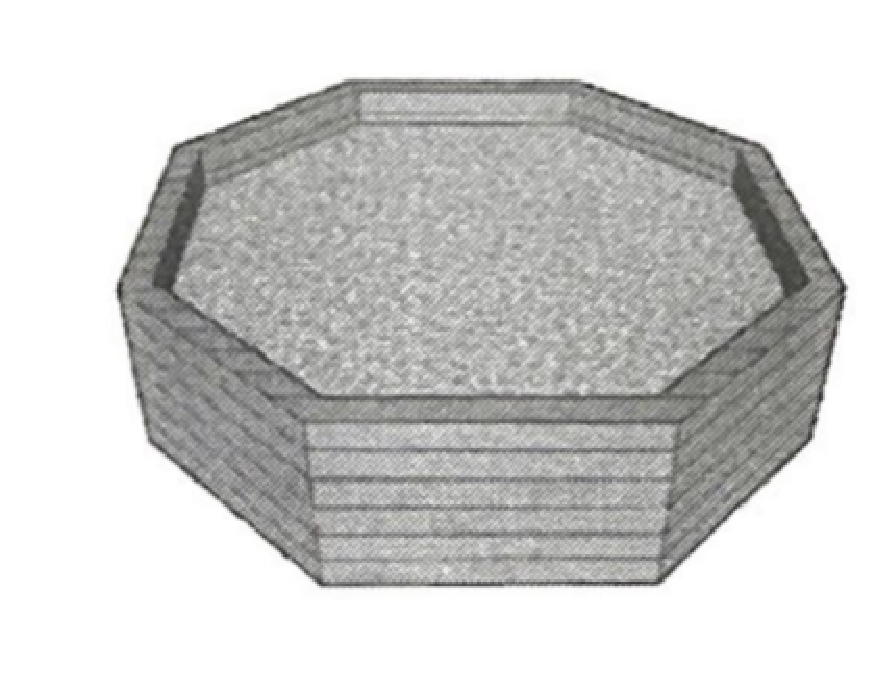
\includegraphics[width=3.5cm]{piscine.eps}
\end{minipage}

	\begin{enumerate}
		\item  Montrer que le volume d'eau nécessaire est environ égal à $24~\text{m}^3$.
		\item  Sachant que le débit du robinet utilisé pour remplir la piscine est de $12$~ L/min, calculer la
durée de remplissage de ces $24~\text{m}^3$ d'eau.\index{vitesse}

Donner le résultat en heures et minutes.

\emph{Rappel}: 1 m$^3 = \np{1000}$~L.
	\end{enumerate}
\end{enumerate}
%%%%  fin Martinique 3 juillet 2024
\newpage
%%% Polynésie 9 septembre 2024
\phantomsection

\hypertarget{Polynesiesep}{}
\label{Polynesiesep}

\lfoot{\small{Polynésie}}
\rfoot{\small{9 septembre 2024}}
\setlength{\headheight}{13.59999pt}
\marginpar{\rotatebox{90}{\textbf{A. P{}. M. E. P{}.}}}
\pagestyle{fancy}
\thispagestyle{empty}
\begin{center}

{\Large \textbf{\decofourleft~Brevet des collèges Polynésie 9 septembre 2024~\decofourright}}

\bigskip

\textbf{Durée : 2 heures} 

\medskip

L'annexe est à rendre avec la copie.
\end{center}

\bigskip

\begin{tabularx}{\linewidth}{|>{\textbf{}}X|}\hline
\multicolumn{1}{|c|}{Indications portant sur l'ensemble du sujet}\\
Toutes les réponses doivent être justifiées, sauf si une indication contraire est donnée.\\
Pour chaque question, si le travail n'est pas terminé, laisser tout de même une trace de la recherche; elle sera prise en compte dans la notation.\\ \hline
\end{tabularx}

\bigskip

\textbf{\large{}Exercice 1 \hfill 21 points}

\medskip

\emph{Dans cet exercice, toutes les questions sont indépendantes.}

\medskip

\begin{enumerate}
\item On a décomposé ci-dessous cinq nombres en produits de facteurs premiers.\index{produit de facteurs premiers}

Parmi ces nombres, lesquels sont divisibles par 21 ?\index{diviseur}

\begin{center}
\renewcommand{\arraystretch}{1.6}
\begin{tabularx}{\linewidth}{|*{5}{>{\centering \arraybackslash}X|}}\hline
Nombre 1& Nombre 2& Nombre 3& Nombre 4& Nombre 5\\ \hline
$2^2 \times 11 \times 23$ &$2^4 \times 3^4 \times 11$	&$7^3 \times 13 \times 17$
&$2 \times 3 \times 5 \times 7$&$2^3 \times 3^2 \times 7$\\ \hline
\end{tabularx}
\end{center}

\item Donner, sans justification, l'écriture scientifique du nombre \np{0,00000276}.

\item La comète Hale-Bopp a atteint la vitesse de \np{2640} km/min. Quelle est sa vitesse en m/s ? \index{vitesse}

\item Quelles sont les solutions de l'équation 
\[(2x - 7)(3x + 1) = 0 \:?\]\index{equation-produit@équation-produit}

\item On considère la fonction $f$ définie par $f(x) = 5x^2 + 2$.

Quelle est l'image de $-3$ par la fonction $f$ ?\index{image}
\end{enumerate}
\begin{minipage}{0.51\linewidth}
\begin{enumerate}[resume]
\item Sur la figure ci-contre (qui n'est pas à l'échelle) :
\begin{itemize}[label=$\bullet~$]
\item les points A, E et C sont alignés;
\item les points B, D et C sont alignés;
\item les droites (AB) et (ED) sont parallèles;
\item AB $= 5$ cm, BD $= 1$ cm, CD$= 3$ cm.
\end{itemize}\index{Thalès}

Calculer DE.
\end{enumerate}
\end{minipage}\hfill
\begin{minipage}{0.46\linewidth}
\psset{unit=1cm}
\begin{pspicture}(6.6,4.4)
\pspolygon(0.4,2.2)(4.8,3.7)(6.2,0.4)%ABC
\psline(1.72,1.8)(5.1,3)
\uput[l](0.4,2.2){A} \uput[u](4.8,3.7){B} \uput[dr](6.2,0.4){C} \uput[r](5.1,3){D}
\uput[dl](1.72,1.8){E}
\uput[u](2.6,2.95){5 cm} \uput[r](4.95,3.35){1 cm} \uput[r](5.65,1.7){3 cm}
\end{pspicture}
\end{minipage}

%\bigskip
\newpage

\textbf{\large{}Exercice 2 \hfill 20 points}

\medskip

On a relevé dans une feuille de calcul les températures maximales Tmax (en \degres C) atteintes à Strasbourg le 25 juin de chaque année de 2010 à 2018 (source : meteociel.fr).

\begin{center}
\begin{tabularx}{\linewidth}{|>{\centering\arraybackslash\cellcolor{lightgray}} c|c|*{9}{>{\centering \arraybackslash}X|}}\hline
\rowcolor{lightgray}	&A			&B		&C&D&E&F&G&H&I&J\\ \hline
1	&Année		&2010 	&2011	&2012	&2013	&2014	&2015	&2016	&2017	&2018\\ \hline
2	&Tmax		& 29 	&$23,1$	& $22,6$	&$17,4$	&$23,4$	&$25,7$	&$25,2$	&26		&24\\ \hline
3	&			&		&		&		&		&		&		&		&		&\\ \hline
4	&Moyenne	&		&		&		&		&		&		&		&		&\\ \hline
5	&Médiane	&24		&		&		&		&		&		&		&		&\\ \hline
6	&Étendue	&$11,6$	&		&		&		&		&		&		&		&\\ \hline
\end{tabularx}
\end{center}

\medskip

\begin{enumerate}
\item On a oublié de calculer la moyenne de cette série.\index{moyenne}

Quelle formule peut-on saisir dans la cellule B4 pour que ce calcul soit effectué ? \index{tableur}
\item Donner, sans détailler les calculs, une valeur approchée au degré Celsius près de la moyenne de la série.
\item Donner une interprétation de la médiane de cette série.\index{médiane}
\item Pour cette question seulement, on considère la série des températures maximales atteintes à Strasbourg le 25 juin de chaque année de 2010 à 2019. 

On sait que l'étendue des températures de cette nouvelle série est égale à $18,5\degres$~C.\index{etendue@étendue}

Déterminer la température maximale atteinte à Strasbourg le 25 juin 2019.\index{maximum}
\end{enumerate}
\medskip

Les questions suivantes portent sur la série des températures maximales atteintes à Strasbourg le 25 juin de chaque année de 2010 à 2018.

\medskip

\begin{enumerate}[resume]
\item  On crée 9 fiches, une par année, sur lesquelles figure la température maximale atteinte le 25 juin de l'année. On prend une fiche au hasard. Chacune des fiches a la même probabilité d'être tirée.
	\begin{enumerate}
		\item Quelle est la probabilité que la température écrite sur cette fiche soit égale à $26\degres$~C ?\index{probabilités}
		\item Quelle est la probabilité que la température écrite sur cette fiche soit inférieure ou égale à 24$\degres$~C?
		\item A-t-on raison de dire que l'on a plus de 40\,\% de chance de prendre une fiche sur laquelle la température est supérieure à $25\degres$~C?
	\end{enumerate}
\end{enumerate}

\newpage

\textbf{\large{}Exercice 3 \hfill 17 points}

\medskip

\begin{minipage}{0.58\linewidth}
Sur la figure ci-contre, qui n'est pas à l'échelle,
\begin{itemize}[label=$\bullet~$]
\item le triangle ONM est rectangle en N,
\item le triangle OPQ est rectangle en P{},
\item le triangle ORS est rectangle en R,
\item ON $= 6$ cm et $\widehat{\text{MON}} = 32\degres$.
\item P est un point du segment [OM] et R est un point du segment [OQ].
\end{itemize}
\end{minipage}\hfill
\begin{minipage}{0.42\linewidth}
\psset{unit=1.1cm}
\begin{pspicture}(4.5,4.1)
%\psgrid
\pspolygon(0.3,1.3)(0.3,3.6)(4.1,3.6)%%MNO
\psline(0.82,1.62)(1.7,0.3)(4.1,3.6)%PQO
\psline(3.04,2.18)(3.65,1.7)(4.1,3.6)%RSO
\psframe(0.3,3.6)(0.5,3.4)\rput{-57}(0.82,1.62){\psframe(0.2,0.2)}
\rput{-38}(3.04,2.18){\psframe(0.2,0.2)}
\psarc(4.1,3.6){0.8}{180}{212}
\uput[d](0.3,1.3){M} \uput[ul](0.3,3.6){N} \uput[ur](4.1,3.6){O}
\uput[d](0.78,1.62){P} \uput[d](1.7,0.3){Q} \uput[d](3.09,2.18){R}
\uput[d](3.65,1.7){S} \uput[u](2.2,3.6){6 cm} \rput(3.65,3.45){\footnotesize $32\degres$}
\end{pspicture}
\end{minipage}

\medskip

\begin{enumerate}
\item Calculer la mesure de la longueur MN. On donnera une valeur approchée au millimètre près.\index{Pythagore}
\item On donne PQ $= 2,5$ cm et OQ $= 6,5$ cm. Montrer que OP $= 6$ cm.
\item Montrer que les triangles ONM et OPQ ne sont pas des triangles égaux.
\item Sachant que le triangle OPQ est un agrandissement du triangle ORS et que OS $= 3,25$ cm, calculer l'aire du triangle ORS.\index{Thalès}
\end{enumerate}


\bigskip

\textbf{\large{}Exercice 4 \hfill 19 points}

\medskip

\begin{enumerate}
\item Sur la figure ci-dessous, DEFGH est un pentagone régulier et le point E appartient à la demi-droite [D$y$). On admet que tous les angles du pentagone régulier mesurent $108$ degrés.

\begin{center}
\psset{unit=1cm}
\begin{pspicture}(-2,-2)(3.5,2.1)
\pspolygon(1.7;18)(1.7;90)(1.7;162)(1.7;234)(1.7;306)%FGHDE
\uput[dl](1.7;234){D} \uput[d](1.7;306){E} \uput[r](1.7;18){F}
\uput[u](1.7;90){G} \uput[l](1.7;162){H} \uput[d](3.2,-1.39){$y$}
\psline(1.7;306)(3.3,-1.39)
\psarc(1.7;306){0.7}{0}{72}
\end{pspicture}
\end{center}

\medskip

Justifier que l'angle $\widehat{\text{FE}y}$ mesure $72$ degrés.\index{calcul d'angle}
\item Dans la suite de cet exercice, aucune justification n'est attendue.
	\begin{enumerate}
		\item Compléter le bloc \og pentagone \fg{} en ANNEXE, à rendre avec la copie, pour obtenir un pentagone régulier. La variable \og longueur \fg{} permet de modifier la longueur des côtés du pentagone.\index{Scratch}
		\item Camille, Lou et Zoé ont chacun codé un programme qui trace un pentagone et son image par l'une des transformations suivantes : translation, symétrie centrale, rotation.\index{symétrie centrale}\index{rotation}\index{translation}

\begin{center}
\begin{tabularx}{\linewidth}{|*{3}{X|}}
\hline
Programme de Camille&Programme de Lou&Programme de Zoé\\ 
\hline
\begin{scratch}[num blocks,scale=0.8]
\blockinit{Quand \greenflag est cliqué}
\blockpen{effacer tout}
\blockmove{aller à x : \ovalnum{0} y : \ovalnum{0}}
\blockmove{s'orienter à ~\ovalnum{90}}
\blockvariable{mettre \selectmenu{longueur} à \ovalnum{60}}
\blockmoreblocks{pentagone}
\blockmove{avancer de \ovalnum{120} pas}
\blockmoreblocks{pentagone}
\end{scratch}
&
\begin{scratch}[num blocks,scale=0.8]
\blockinit{Quand \greenflag est cliqué}
\blockpen{effacer tout}
\blockmove{aller à x : \ovalnum{0} y : \ovalnum{0}}
\blockmove{s'orienter à ~\ovalnum{90}}
\blockvariable{mettre \selectmenu{longueur} à \ovalnum{60}}
\blockmoreblocks{pentagone}
\blockmove{tourner \turnleft{} de \ovalnum{60} degrés}
\blockmoreblocks{pentagone}
\end{scratch}
&
\begin{scratch}[num blocks,scale=0.8]
\blockinit{Quand \greenflag est cliqué}
\blockpen{effacer tout}
\blockmove{aller à x : \ovalnum{0} y : \ovalnum{0}}
\blockmove{s'orienter à ~\ovalnum{90}}
\blockvariable{mettre \selectmenu{longueur} à \ovalnum{60}}
\blockmoreblocks{pentagone}
\blockmove{tourner \turnleft{} de \ovalnum{180} degrés}
\blockmoreblocks{pentagone}
\end{scratch}\\ 
\hline
\end{tabularx}
\end{center}

On rappelle que l'instruction \og s'orienter à 90 \fg{} signifie que l'on s'oriente vers la droite.

Les trois élèves ont effectué une copie d'écran de ce qu'ils ont obtenu sans indiquer ni leur
prénom ni le nom de la transformation choisie.

\begin{center}
\begin{tabularx}{\linewidth}{|*{3}{X|}}\hline
Copie d'écran 1 &Copie d'écran 2& Copie d'écran 3\\ \hline
\begin{center}
\psset{unit=0.75cm}
\begin{pspicture}(-2,-2)(2,2)
\def\penta{\pspolygon(1.;18)(1.;90)(1.;162)(1.;234)(1.;306)}
\rput{-12}(-0.3945,0.1045){\penta}\rput(0.6,0.){\penta}
\end{pspicture}
\end{center}
&
\begin{center}
\psset{unit=0.75cm}
\begin{pspicture}(-2,-2)(2,2)
\def\penta{\pspolygon(1.;18)(1.;90)(1.;162)(1.;234)(1.;306)}
\rput(0.6,0.6){\penta}\rput{180}(-0.6,-1){\penta}
\end{pspicture}
\end{center}
&
\begin{center}
\psset{unit=0.75cm}
\begin{pspicture}(-2,-2)(2,2)
\def\penta{\pspolygon(1.;18)(1.;90)(1.;162)(1.;234)(1.;306)}
\rput(-1.2,0){\penta}\rput(1.2,0){\penta}
\end{pspicture}
\end{center}\\ \hline
\end{tabularx}
\end{center}

Compléter le tableau en ANNEXE, à rendre avec la copie, en associant le prénom de l'élève au numéro de sa copie d'écran ainsi qu'au nom de la transformation qu'il a choisie.
\item Sofia souhaite illustrer à l'aide d'un programme l'effet d'une homothétie sur un pentagone. 

Le tableau en ANNEXE donne, dans le désordre, toutes les instructions utiles pour écrire ce programme. L'ordre d'apparition dans le programme de deux instructions est précisé.

Compléter ce tableau sur l'ANNEXE, à rendre avec la copie, en indiquant l'ordre d'apparition de chacune des instructions dans le programme de Sofia.
	\end{enumerate}
\end{enumerate}

%\bigskip
\newpage

\textbf{\large{}Exercice 5 \hfill 23 points}

\medskip

La piscine du camping \og le Rocher\fg{} dispose d'un bassin circulaire de forme cylindrique de rayon $3,60$~m et de hauteur $1,50$~m. En fin de saison, on utilise une pompe dont le débit est de $14,1$~m$^3$/h pour vider l'eau de la piscine.

\medskip

\begin{enumerate}
\item Montrer que le volume du bassin, arrondi au dixième de m$^3$, est 61,1m$^3$.\index{volume d'un cylindre}
\item Le bassin est plein. On met en route la pompe. Au bout de 2 heures, quel volume d'eau en m$^3$ reste-t-il à vider ?\index{vitesse}
	\end{enumerate}

On considère la fonction $V\::\: t \longmapsto  61,1 - 0,235 t$.

	\begin{enumerate}[resume]
\item 
	\begin{enumerate}
		\item Montrer que l'expression $V(t)$ permet de déterminer le volume d'eau en m$^3$ qu'il reste à vider dans le bassin en fonction de la durée $t$, exprimée en minute, d'utilisation de la pompe.
		\item Calculer le temps nécessaire pour que le volume d'eau restant à vider soit égal à $30$ m$^3$.
		
On donnera une valeur approchée à la minute près.\index{vitesse}
	\end{enumerate}
	
\item On a tracé ci-dessous une partie de la représentation graphique de la fonction $V$.

\begin{center}
\psset{unit=0.04cm,arrowsize=3pt 3}
\begin{pspicture*}(-20,-20)(330,120)
\psgrid[unit=2cm,subgriddiv=5,gridlabels=0,gridcolor=gray,subgridcolor=lightgray](-1,-1)(7,3)
\psaxes[linewidth=1.25pt,Dx=50,Dy=50,labelFontSize=\scriptstyle]{->}(0,0)(-20,-20)(330,120)
%\multido{\n=0+10}{32}{\psline[linewidth=0.1pt](\n,0)(\n,110)}
%\multido{\n=0+10}{12}{\psline[linewidth=0.1pt](0,\n)(330,\n)}
%\multido{\n=0+50}{6}{\psline[linewidth=0.7pt](\n,0)(\n,110)}
%\multido{\n=0+50}{3}{\psline[linewidth=0.7pt](0,\n)(330,\n)}
\psplot[plotpoints=2000,linewidth=1.25pt,linecolor=blue]{-20}{330}{61.1 0.235 x mul sub}
\uput[u](305,0){$t$}\uput[r](0,105){$V(t)$}
\end{pspicture*}
\end{center}

Répondre aux questions suivantes par une lecture graphique.\index{lecture graphique}
	\begin{enumerate}
		\item Déterminer l'antécédent de 40 par la fonction $V$. Interpréter le résultat.\index{antécédent}
		\item Déterminer le temps nécessaire pour que la pompe vide complètement le bassin.
	\end{enumerate}
\end{enumerate}

\newpage

\begin{center}\textbf{\large ANNEXE}\end{center}

\medskip

\textbf{Exercice 4}

\vspace{1cm}

\begin{tabular}{c c c}
\textbf{Question 2. a.}&&\textbf{Question 2. b.}\\%[7pt]
\\
\begin{scratch}[scale=1]
\initmoreblocks{définir \namemoreblocks{pentagone}}
\blockpen{stylo en position d'écriture}
\blockrepeat{répéter \ovalnum{\hspace*{0.7cm}} fois}
{\blockmove{avancer de \ovalnum{longueur} pas}
\blockmove{tourner \turnleft{} de \ovalnum{\hspace*{0.7cm}} degrés}
}
\blockpen{relever le stylo}
\end{scratch}
&&
{\renewcommand{\arraystretch}{1.6}
\begin{tabular}[t]{|m{1.5cm}|m{1.3cm}|m{3.5cm}|}
\multicolumn{3}{c}{~~}\\
\hline
Nom de\newline l'élève&Numéro\newline de la\newline copie d'écran&Nom de la\newline transformation\\ \hline
Camille&&\\ \hline 
Lou &&\\ \hline 
Zoé&&\\ \hline 
\end{tabular}}\\
\end{tabular}

\vspace{1cm}

\textbf{Question 2. c.}

\bigskip

\begin{center}
\begin{tabular}{|l| p{7cm}|}\hline
Instruction&Ordre d'apparition de l'instruction dans le programme de Sofia\\ \hline
\begin{scratch}[scale=0.8]\blockpen{effacer tout} \end{scratch}&\\ \hline
\begin{scratch}[scale=0.8]\blockmove{s'orienter à \ovalnum{90} } \end{scratch}&\\ \hline
\begin{scratch}[scale=0.8]\blockmoreblocks{pentagone} \end{scratch}&\multicolumn{1}{|c|}{6\up{e}}\\ \hline
\begin{scratch}[scale=0.8]\blockinit{Quand \greenflag est cliqué} \end{scratch}&\multicolumn{1}{|c|}{1\up{re}}\\ \hline
\begin{scratch}[scale=0.8]\blockvariable{mettre \selectmenu{longueur} à \ovalnum{60}} \end{scratch}&\\ \hline
\begin{scratch}[scale=0.8]\blockmove{aller à x : \ovalnum{0} y : \ovalnum{0}} \end{scratch}&\\ \hline
\begin{scratch}[scale=0.8]\blockmoreblocks{pentagone} \end{scratch}&\\ \hline
\begin{scratch}[scale=0.8]\blockvariable{mettre \selectmenu{longueur} à \ovaloperator{\ovalvariable{longueur} *\ovalnum{1.5}}} \end{scratch}&\\ \hline
\end{tabular}
\end{center}
%%%%%%%%  fin Polynésie septembre 2024
\newpage
%%%%%%%%  Métropole Antilles Guyane Mayotte 19 septembre 2024
\phantomsection

\hypertarget{Metropolesep}{}
\label{Metropolesep}

\thispagestyle{empty}
\lfoot{\small{Métropole Antilles Guyane Mayotte}}
\rfoot{\small{19 septembre 2024}}

\begin{center} {\Large \textbf{\decofourleft~Brevet Métropole Antilles--Guyane 19 septembre 2024 \decofourright}}
	\end{center}

\begin{tabularx}{\linewidth}{|X|}\hline
\multicolumn{1}{|c|}{Indications portant sur l'ensemble du sujet}\\
Toutes les réponses doivent être justifiées, sauf si une indication contraire est donnée.\\
Pour chaque question, si le travail n'est pas terminé, laisser tout de même une trace de la recherche ; elle sera prise en compte dans la notation.\\ \hline
\end{tabularx}

\bigskip

{\large \textbf{Exercice 1 \hfill 20 points}}

\medskip

Pour chacune des affirmations suivantes, dire si elle est vraie ou fausse.

Toutes les réponses devront être justifiées.

\medskip

\begin{enumerate}
\item \textbf{Affirmation 1}

La décomposition en produit de facteurs premiers du nombre $260$ est $4 \times 5 \times 13$.\index{produit de facteurs premiers}
\item \textbf{Affirmation 2}

Une urne opaque contient des boules indiscernables au toucher: 3 boules blanches, 4 boules jaunes et 8 boules rouges.

On pioche au hasard une boule dans cette urne et on note sa couleur.

Une autre urne opaque contient des boules indiscernables au toucher : 1 boule marquée de la lettre A, 1 boule marquée de la lettre B et 3 boules marquées de la lettre C.

On pioche au hasard une boule dans cette urne et on note la lettre obtenue.

La probabilité d'obtenir une boule de couleur rouge est supérieure à la probabilité d'obtenir une boule marquée de la lettre C.\index{probabilités}
\item \textbf{Affirmation 3}

La solution de l'équation $7x + 5 = 2x - 2$ est $-1,4$.\index{résolution d'équation}
\item \textbf{Affirmation 4}

On empile 10 pièces cylindriques de $1,9$~cm de diamètre et de $0,2$~cm de hauteur. Le volume du cylindre, arrondi à l'unité, formé par les $10$~pièces est de $6$~cm$^3$.\index{volume d'un cylindre}

\emph{Rappel} : le volume d'un cylindre de rayon $R$ et de hauteur $h$ est égal à $\pi \times R^2 \times h$.
\item \textbf{Affirmation 5}

Un éléphant qui court à une vitesse de 5 m/s est plus rapide qu'un cochon qui se déplace à une vitesse de 17 km/h.\index{vitesse}
\end{enumerate}

\newpage

{\large \textbf{Exercice 2 \hfill 20 points}}

\medskip

\begin{minipage}{0.5\linewidth}
Un agriculteur possède un champ de blé ayant la forme
d'un triangle ABC rectangle en B représenté ci-contre.

On donne AB $= 200$ m et BC $= 150$ m.

Pour moissonner son champ, il utilise une moissonneuse batteuse qui, à chaque passage, coupe
des bandes de 12 mètres de large parallèles à la droite (AB). On a donc BE~$=~12$~m.

Il commence à passer le long du côté [AB]. Le segment en pointillés [DE] représente la limite du premier passage de la moissonneuse batteuse.

Après avoir fait 5 passages, il a moissonné le quadrilatère ABGF{}.

\medskip

\begin{enumerate}
\item 
	\begin{enumerate}
		\item Montrer que BG $= 60$ m.
		\item En déduire que CG $= 90$ m.
	\end{enumerate}	
\item Démontrer que la longueur GF est de $120$ m.
\end{enumerate}
\end{minipage}\hfill
\begin{minipage}{0.45\linewidth}
\psset{unit=1cm}
\begin{pspicture}(6.2,10.2)
%\psgrid
\pspolygon(0.1,0.2)(6.1,0.2)(0.1,10.3)
\uput[dr](6.1,0.2){C}
\psline(2.4,0.2)(2.4,6.4)
\psline[linestyle=dashed](0.56,0.2)(0.56,9.5)
\psline[linestyle=dashed](1.02,0.2)(1.02,8.8)
\psline[linestyle=dashed](1.48,0.2)(1.48,8)
\psline[linestyle=dashed](1.94,0.2)(1.94,7.2)
\multido{\n=0.33+0.46}{5}{\rput(\n,0.2){/}}
\uput[ul](0.1,10.3){A}\uput[dl](0.1,0.2){B}\psframe(0.1,0.2)(0.3,0.4)\psframe(2.4,0.2)(2.6,0.4)
\uput[d](0.56,0.2){E}\uput[ur](0.56,9.5){D}
\uput[d](2.4,0.2){G}\uput[ur](2.4,6.4){F}
\end{pspicture}
\end{minipage}

\begin{enumerate}[start=3]
\item
	\begin{enumerate}
		\item Démontrer que l'aire du triangle rectangle CGF est de \np{5400}~m$^2$.\index{aire d'un triangle}
		\item Le quadrilatère ABGF a une surface de \np{9600} m$^2$ qui a été moissonnée en 80 minutes.
		
On admet que le temps de travail de la moissonneuse batteuse est proportionnel à la surface moissonnée.

Calculer le temps de travail qu'il faut pour moissonner la partie restante CGF de son champ.\index{proportionnalité}
	\end{enumerate}
\item L'année suivante, il décide de clôturer son champ ABC afin d'y mettre des animaux pour l'été. Quelle longueur de clôture doit-il acheter ?\index{Thalès}
\end{enumerate}

\bigskip

{\large \textbf{Exercice 3\hfill 20 points}}

\medskip

Une entreprise décide de faire poser sur le toit de son hangar des panneaux solaires.

Pendant une semaine d'utilisation, les productions d'électricité journalières en kilowattheures (kWh) de ces panneaux ont été relevées dans le tableau ci-dessous :

\begin{center}
\begin{tabularx}{\linewidth}{|m{2cm}|*{7}{>{\centering \arraybackslash}X|}}\hline
Jour de la semaine&Lundi&Mardi& Mercredi& Jeudi&Vendredi& Samedi&\small Dimanche\\ \hline
Production d'électricité en kWh&381&363 &322& 329&393& 405& 376\\ \hline
\end{tabularx}
\end{center}

\smallskip

\begin{enumerate}
\item
	\begin{enumerate}
		\item Quel jour la production d'électricité a-t-elle été la plus grande ?
		\item Calculer l'étendue de ces productions d'électricité.\index{etandue@étendue}
		\item Quelle est la production moyenne d'électricité par jour sur cette période ?\index{moyenne}
	\end{enumerate}
\item L'entreprise revend 15\,\% de sa production d'électricité au tarif de 8 centimes le kWh.\index{pourcentage}

Combien a-t-elle gagné en euros pendant ces 7 jours ?
\item Afin que les panneaux solaires aient une production maximale, le toit doit avoir une pente avec l'horizontale comprise entre $30\degres$ et $35\degres$.

\begin{minipage}{0.35\linewidth}
Schéma en coupe du hangar.

La pente du toit avec l'horizontale correspond à l'angle $\widehat{\text{OLV}}$.\index{calcul d'angle}

\end{minipage}\hfill
\begin{minipage}{0.62\linewidth}
\psset{unit=1cm,arrowsize=2pt 3}
\begin{pspicture}(8.5,6.6)
%\psgrid
\pspolygon(2,0)(8.2,0)(8.2,3.9)(5.1,6.3)(2,3.9)
\psline(5.1,6.3)(5.1,3.9)\psframe(5.1,3.9)(5.3,4.1)
\psline(8.2,3.9)(2,3.9)
\psline[linewidth=2.5pt](4.7,6)(2.4,4.2)
\uput[d](5.1,3.9){V} \uput[r](8.2,3.9){K} \uput[u](5.1,6.3){O} \uput[l](2,3.9){L} 
\uput[r](5.1,5.1){7 m}\rput{37}(3.56,5.4){13,5 m}
\rput(1.8,5.8){panneaux solaires}\psline[linewidth=1.2pt]{->}(1.8,5.5)(3.2,4.9)
\end{pspicture}
\end{minipage}

\medskip

Sur ce toit, les panneaux solaires ont-ils une production maximale?

\bigskip

\end{enumerate}
{\large \textbf{Exercice 4 \hfill 20 points}}

\medskip

On considère la fonction $f$ définie par 

\[f(x) = x^2 + 10x + 16.\]\index{polynôme}

\begin{enumerate}
\item Vérifier par le calcul que l'image de 6 par la fonction $f$ est $112$.\index{image}
\item On utilise un tableur afin de calculer les images des entiers compris entre $-4$ et 4 par la
fonction $f$.

\begin{center}
\begin{tabularx}{\linewidth}{|c|*{10}{>{\centering \arraybackslash}X|}}\hline
&A&B&C&D&E&F&G&H&I&J\\ \hline
1&$x$&$-4$&$-3$&$-2$&$-1$&0&1&2&3&4\\ \hline
2&$f(x)$&$-8$&$-5$&0&7&16&27&40&55&72\\ \hline
\end{tabularx}
\end{center}

	\begin{enumerate}
		\item Parmi les 4 formules ci-dessous, recopier celle qui a été saisie dans la cellule B2, puis
étirée vers la droite afin de calculer les images des nombres donnés par la fonction $f$.\index{tableur}

\begin{footnotesize}
\fbox{=B1*B1+10*B1+16}\, \fbox{=A1*A1+10*A1+16}\, \fbox{$=(-4)*(-4)+10*(-4)+16$} \, \fbox{$=x*x+10*x+16$}
\end{footnotesize}
		\item En utilisant le tableau, déterminer un antécédent de $0$.\index{antécédent}
	\end{enumerate}
\item
	\begin{enumerate}
		\item Démontrer que $f(x)$ peut s'écrire $(x + 2)(x + 8)$.\index{développement}
		\item En déduire un autre antécédent de 0 par la fonction $f$.
	\end{enumerate}
\end{enumerate}

\bigskip

{\large \textbf{Exercice 5 \hfill 20 points}}

\medskip

La quadrilatère ABCD ci-dessous est constitué de deux triangles équilatéraux de côté 5 cm.\index{triangle équilatéral}

\psset{unit=0.75cm}
\begin{center}
\begin{pspicture}(6.5,5)
%\psgrid
\pspolygon(0.2,0.2)(5.2,0.2)(7.5,4.53)(2.7,4.53)%BCDA
\psline(5.2,0.2)(2.7,4.53)
\uput[ul](2.7,4.53){A} \uput[dl](0.2,0.2){B} \uput[dr](5.2,0.2){C} \uput[ur](7.5,4.53){D} \uput[d](2.7,0.2){5 cm}
\psline(2.7,0.3)(2.7,0.1)
\def\marque{\psline(0,0.1)(0,-0.1)}
\rput{60}(1.45,2.36){\marque}\rput{-60}(3.95,2.36){\marque}\rput{60}(6.35,2.36){\marque}
\rput(5.1,4.53){\marque}
\end{pspicture}
\end{center}

\medskip

\begin{enumerate}
\item
	\begin{enumerate}
		\item Reproduire le quadrilatère ABCD en vraie grandeur.
		\item Quelle est sa nature ?\index{losange}
		\item Démontrer que l'angle $\widehat{\text{BCD}}$ mesure $120\degres$.\index{calcul d'angle}
	\end{enumerate}	
\item Le programme ci-dessous permet de créer le bloc Motif qui trace le quadrilatère ABCD.

Recopier et compléter les lignes 5 et 6 de ce programme.\index{Scratch}

On utilise l'échelle suivante : 10 pas dans le programme représentent 1 cm dans la réalité.

\medskip

\begin{minipage}{0.55\linewidth}
\begin{scratch}[scale=0.75,num blocks]
\renewcommand*\numblock[1]{\large #1~~}
\initmoreblocks{d\'efinir \namemoreblocks{Motif}}
\blockrepeat{r\'ep\'eter \ovalnum{2} fois}
{
\blockmove{avancer de \ovalnum{50 } pas}
\blockmove{tourner \turnleft{} de \ovalnum{60} degr\'es}
\blockmove{avancer de \ovalnum{\ldots } pas}
\blockmove{tourner \turnleft{} de \ovalnum{\ldots} degr\'es}
}
\end{scratch}
\end{minipage}\hfill
\begin{minipage}{0.45\linewidth}
\psset{unit=0.5cm,arrowsize=2pt 3}
\def\losan{\pspolygon(0.2,0.2)(5.2,0.2)(7.5,4.53)(2.7,4.53)}
\psset{unit=0.25cm,arrowsize=2pt 3}
\begin{pspicture}(4,3.8)
\rput(1.3,2.){\losan}
\rput(1.3,-2.4){Point de départ}
\psline[linecolor=blue]{->}(1.3,-1.4)(1.3,2)
\end{pspicture} 

\end{minipage}

\item Recopier et compléter les trois phrases suivantes afin d'associer chaque figure au programme qui permet de la tracer.

Le programme A permet de tracer la figure \ldots.

Le programme B permet de tracer la figure \ldots.

Le programme C permet de tracer la figure \ldots.
\end{enumerate}

\medskip

\begin{center}
\psset{linecolor=blue}
\begin{tabularx}{\linewidth}{*{3}{>{\centering \arraybackslash}X}}
\fbox{Programme A} & \fbox{Programme B} & \fbox{Programme C}\\
& & \\
\begin{scratch}[scale=0.75]
\blockinit{quand \greenflag est cliqu\'e}
\blockmove{aller à x: \ovalnum{0} y: \ovalnum{0}}
\blockmove{s'orienter à \ovalnum{90}}
\blockpen{effacer tout}
\blockpen{stylo en position d'\'ecriture}
\blockrepeat{r\'ep\'eter \ovalnum{5} fois}
{
\blockevent{Motif}
\blockmove{tourner \turnleft{} de \ovalnum{72} degr\'es}
}
\end{scratch}
&
\begin{scratch}[scale=0.75]
\blockinit{quand \greenflag est cliqu\'e}
\blockmove{aller à x: \ovalnum{0} y: \ovalnum{0}}
\blockmove{s'orienter à \ovalnum{90}}
\blockpen{effacer tout}
\blockpen{stylo en position d'\'ecriture}
\blockrepeat{r\'ep\'eter \ovalnum{5} fois}
{
\blockevent{Motif}
\blockmove{tourner \turnleft{} de \ovalnum{72} degr\'es}
\blockmove{avancer de \ovalnum{25 } pas}
}
\end{scratch}
&
\begin{scratch}[scale=0.75]
\blockinit{quand \greenflag est cliqu\'e}
\blockmove{aller à x: \ovalnum{0} y: \ovalnum{0}}
\blockmove{s'orienter à \ovalnum{90}}
\blockpen{effacer tout}
\blockpen{stylo en position d'écriture}
\blockrepeat{r\'ep\'eter \ovalnum{5} fois}
{
\blockevent{Motif}
\blockmove{avancer de \ovalnum{25 } pas}
}
\end{scratch}\\
&& \\
&& \\
Figure 1&Figure 2&Figure 3\\
\psset{unit=0.25cm}
\def\losan{\pspolygon(-1.8,7.2)(3.2,7.2)(5.7,11.53013)(0.7,11.53013)}
\begin{pspicture}(0,0)(2.5,10)
\multido{\n=-5+2.5}{5}{\rput(\n,0){\losan}}
\end{pspicture}
&
\psset{unit=0.25cm}
\def\losan{\pspolygon(-1.8,0.2)(3.2,0.2)(5.7,4.53013)(0.7,4.53013)}
\begin{pspicture}(-2,-10)(2,10)
\def\losan{\pspolygon(0,0)(5,0)(7.5,4.33013)(2.5,4.33013)}
\multido{\n=0+72}{5}{\rput{\n}(0,0){\losan}}
\end{pspicture}
&
\psset{unit=0.25cm}
\def\losan{\pspolygon(0,0)(5,0)(7.5,4.33013)(2.5,4.33013)}
\begin{pspicture}(-7,-10)(4,12)
%\psgrid
\multido{\i=18+72,\I=90+72,\n=72+72}{5}{
\psline(2.13;\i)(2.13;\I)
\rput{\n}(2.13;\i){\losan}}
\end{pspicture}
\\
\end{tabularx}
\end{center}
%%%  fin Métropole Antilles Guyane Mayotte 19 septembre 2024
%%%%   Amérique du Sud 2 décembre 2024
\phantomsection

\hypertarget{AmeriqueSud}{}
\label{AmeriqueSud}

\lfoot{\small{Amérique du Sud}}
\rfoot{\small{2 décembre 2024}}
\pagestyle{fancy}
\thispagestyle{empty}
\begin{center}

{\Large \textbf{\decofourleft~Brevet des collèges Amérique du Sud 2 décembre 2024~\decofourright}}

\bigskip

\textbf{Durée : 2 heures}

\end{center}

\textbf{\large Exercice 1 \hfill 20 points}

\bigskip

Cet exercice est un Q.C.M. (questionnaire à choix multiple).

Pour chacune des cinq questions, trois réponses sont proposées et une seule convient.

Pour chacune des cinq questions, écrire sur la copie le numéro de la question et la lettre correspondant à la réponse choisie.

\textbf{Aucune justification n'est attendue.}

Une réponse fausse ou l'absence de réponse ne retire pas de point.

\begin{center}
\begin{tabularx}{\linewidth}{|c|m{4.5cm}|*{3}{>{\centering \arraybackslash}X|}}\hline
	&&A&B&C\\ \hline
1	&Une urne contient trois jetons verts et deux jetons blancs. On tire un jeton au hasard.

Quelle est la probabilité d'obtenir un jeton blanc?&
$\dfrac23$&$\dfrac35$&$\dfrac25$\\ \hline
2	&
\psset{unit=0.6cm,arrowsize=2pt 3}
\begin{pspicture}(-1,-1)(5.5,1.3)
\psframe(3,1)\psline(1,1)(1,0)\psline(2,1)(2,0)
\psline(3,0)(3.4,0.35)(3.4,1.35)(3,1)
\psline(3.4,1.35)(3.8,1.7)
\psline{->}(5.5,1)(4,1)
\psline(1,1)(1.4,1.35)(3.4,1.35)
\psline(2,1)(2.8,1.7)(3.8,1.7)(3.8,0.7)(3.4,0.35)
\psline(3.8,0.7)(3.8,-0.3)(3.4,-0.65)(3.4,0.35)
\psline(3.4,-0.65)(2.4,-0.65)(2.4,0)
\psline(1.4,1.35)(1.4,3.35)(0.4,3.35)(0,3)(1,3)(1,1)
\psline(1,3)(1.4,3.35)\psline(0,2)(1,2)(1.4,2.35)
\psline(0,3)(0,1)
\end{pspicture}

Quelle est la vue de droite de ce solide ? 
&
\psset{unit=0.6cm}
\begin{pspicture}(3,5.5)
\psframe(0,1)(1,5)
\psline(0,2)(1,2)\psline(0,3)(1,3)
\psline(1,1)(3,1)(3,2)(1,2)\psline(2,1)(2,0)(3,0)(3,1)\psline(0,4)(1,4)\psline(2,1)(2,2)\end{pspicture}
&
\psset{unit=0.6cm}
\begin{pspicture}(3,5)\psframe(0,1)(1,4) \psframe(0,1)(2,2)\psline(0,3)(1,3)\psline(1,1)(1,0)(2,0)(2,1) \end{pspicture}
&
\psset{unit=0.6cm}
\begin{pspicture}(3,5)\psframe(0,1)(2,2)\psframe(1,0)(2,4)\psline(1,3)(2,3) \end{pspicture}\\ \hline
3&
\psset{unit=0.9cm}
\begin{pspicture}(-0.5,-0.3)(3.5,2.6)
\pspolygon(0.2,2.3)(0.5,0.2)(3.6,0.2)%ABC
\uput[l](0.2,2.3){\footnotesize A} \uput[dl](0.5,0.2){\footnotesize B} \uput[dr](3.6,0.2){\footnotesize C} \uput[ur](1,0.2){\footnotesize D} \uput[l](0.44,0.53){\footnotesize H}
\psline(1,0.2)(0.44,0.53)
\end{pspicture}

 B, H et A sont alignés.

B, D et C sont alignés.

BD = 2 cm ; BC = 10 cm  ; 

AC = 16 cm; (DH) // (AC).

Quelle est la longueur du segment [DH] ?
&3,2 cm&4 cm&4,8 cm\\ \hline

\end{tabularx}
\end{center}


\begin{center}
\begin{tabularx}{\linewidth}{|c|m{4.5cm}|*{3}{>{\centering \arraybackslash}X|}}\hline
&&A&B&C\\ \hline
4& \parbox{4cm}{\centering Voici un engrenage:\rule{0pt}{15pt}\\ \hspace*{3mm}12~dents \hspace*{6mm} 9~dents}
\psset{unit=0.3cm}
\begin{pspicture}(-4.5,-3.5)(10,4.5)
%\psgrid
\def\denta{\psline(2;78)(2;82)(2.3;82)(3;88)(3;92)(2.3;98)(2;98)(2;102)}
\multido{\n=90+30,\na=0+30}{12}{\rput{\na}(0.7;\n){\denta}}
\multido{\i=97+30,\I=113+30}{12}{\psarc(0,0){2.67}{\i}{\I}}
\def\dentb{\psline(1.5;-12)(1.5;-8)(1.725;-8)(2.25;-2)(2.25;2)(1.725;8)(1.5;8)(1.5;12)}
\def\roued{\multido{\n=-5+40,\na=0+40}{9}{\rput{\na}(0.2;\n){\dentb}}}%
\multido{\i=8+40,\I=32+40}{9}{\psarc(5.75,0){1.67}{\i}{\I}}
%\pscircle(0,0){2.57}
%\pscircle(5.75,0){1.6}
\rput(5.75,0){\roued}
\end{pspicture}

 Si la petite roue effectue exactement 4 tours complets, combien de tours complets effectue la grande roue ?&3 tours complets&4 tours complets&6 tours complets\\ \hline
5&\psset{unit=0.7cm}
\begin{center}
\begin{pspicture}(3.3,3.3)
\psframe(2,2)\psframe(2,2)(3,3)
\psline(0,2)(2,0)\psline(2,3)(3,2)
\uput[dl](0,0){\footnotesize F} \uput[d](2,0){\footnotesize E} \uput[l](0,2){\footnotesize G} \uput[ul](2,2){\footnotesize A}
\uput[r](3,2){\footnotesize D} \uput[ur](3,3){\footnotesize C} \uput[ul](2,3){\footnotesize B}
\multido{\n=0+1}{4}{\psline[linewidth=0.2pt](\n,0)(\n,3)}
\multido{\n=0+1}{4}{\psline[linewidth=0.2pt](0,\n)(3.2,\n)}
\end{pspicture}
\end{center}

\medskip

Le carré AGFE est l'image du carré ADCB par une homothétie de centre A.

Le triangle EGF est l'image d'un triangle par cette même homothétie.

Quel est ce triangle ?
&GEA&ABD&BDC\\ \hline
\end{tabularx}
\end{center}

\bigskip

\textbf{\large Exercice 2 \hfill 24 points}

\bigskip

On considère deux fonctions $f$ et $g$ définies par :

\[f(x) = x^2 - x - 6 \qquad \qquad g(x) = -2x.\]

\begin{enumerate}
\item 
	\begin{enumerate}
		\item Montrer que l'image de 5 par la fonction $f$ est 14.
		\item Déterminer l'antécédent de 4 par la fonction $g$.
		\end{enumerate}		
Pour calculer des images de nombres par les fonctions $f$et $g$, on utilise un tableur et on obtient la copie d'écran suivante:

\begin{center}
\begin{tabularx}{0.9\linewidth}{|c|c|*{7}{>{\centering \arraybackslash}X|}}\hline
	&\text{A}&B&C&D&E&F&G&H\\ \hline
1	&$x$&$-4$&$-3$&$-2$&$-1$&0&1&2\\ \hline
2	&$f(x) = x^2 - x - 6$&14&6&0&$-4$&$-6$&$-6$&$-4$\\ \hline
3	&$g(x) = -2x$&8&6&4&2&0&$-2$&$-4$\\ \hline
\end{tabularx}
\end{center}

	\begin{enumerate}[resume]
		\item À l'aide des informations précédentes, citer deux antécédents de 14 par la fonction $f$.
		
		\item  Quelle formule a-t-on pu saisir dans la cellule B2 avant de l'étirer vers la droite jusqu'à la cellule H2 ?
		\item Existe-t-il un nombre qui a la même image par la fonction $f$ et par la fonction $g$ ?
		\end{enumerate}
\item 
	\begin{enumerate}
		\item Montrer que, pour tout nombre $x,\, f(x)$ est égal à $(x + 2)(x - 3)$. 
		\item Résoudre l'équation $f(x) = 0$.
	\end{enumerate}
\end{enumerate}

\bigskip

\textbf{\large Exercice 3 \hfill 22 points}

\medskip

\begin{enumerate}
\item Le tableau ci-dessous présente, pour quatre félins étudiés, les probabilités d'attraper leur proie quand ils la poursuivent.

\begin{center}
\begin{tabularx}{0.75\linewidth}{|*{2}{>{\centering \arraybackslash}X|}}\hline
Félin étudié &
Probabilité d'attraper la proie qu'il poursuit\\ \hline
Le lion&25\,\%\\ \hline
Le guépard&$\dfrac12$\rule[-10pt]{0pt}{28pt}\\ \hline
Le tigre&$0,1$\\ \hline
Le chat à pieds noirs&$\dfrac{6}{10}$\rule[-10pt]{0pt}{28pt}\\ \hline
\end{tabularx}
\end{center}

Vérifier que, parmi les quatre félins étudiés, le chat à pieds noirs a la probabilité la plus élevée d'attraper sa proie quand il la poursuit.
\item  Le plus souvent, le guépard est le félin le plus rapide avec une vitesse pouvant atteindre 115 km/h.
À cette vitesse, en combien de secondes le guépard parcourt-il 100 mètres?
On donnera une valeur approchée au centième de seconde près.

 Dans un pays d'Afrique, on estimait à :

\begin{itemize}[label=$\bullet~$]
\item \np{1200} guépards en 1999.
\item 170 guépards en 2016.
\end{itemize}

Dans ce pays, est-il vrai que le nombre de guépards a baissé d'environ 86\,\% entre 1999 et 2016 ?

\item Dans le parc national d'Etosha en Namibie, on peut observer des lions et des guépards.
À l'aide de la carte ci-dessous, donner approximativement la latitude et la longitude du parc national d'Etosha.

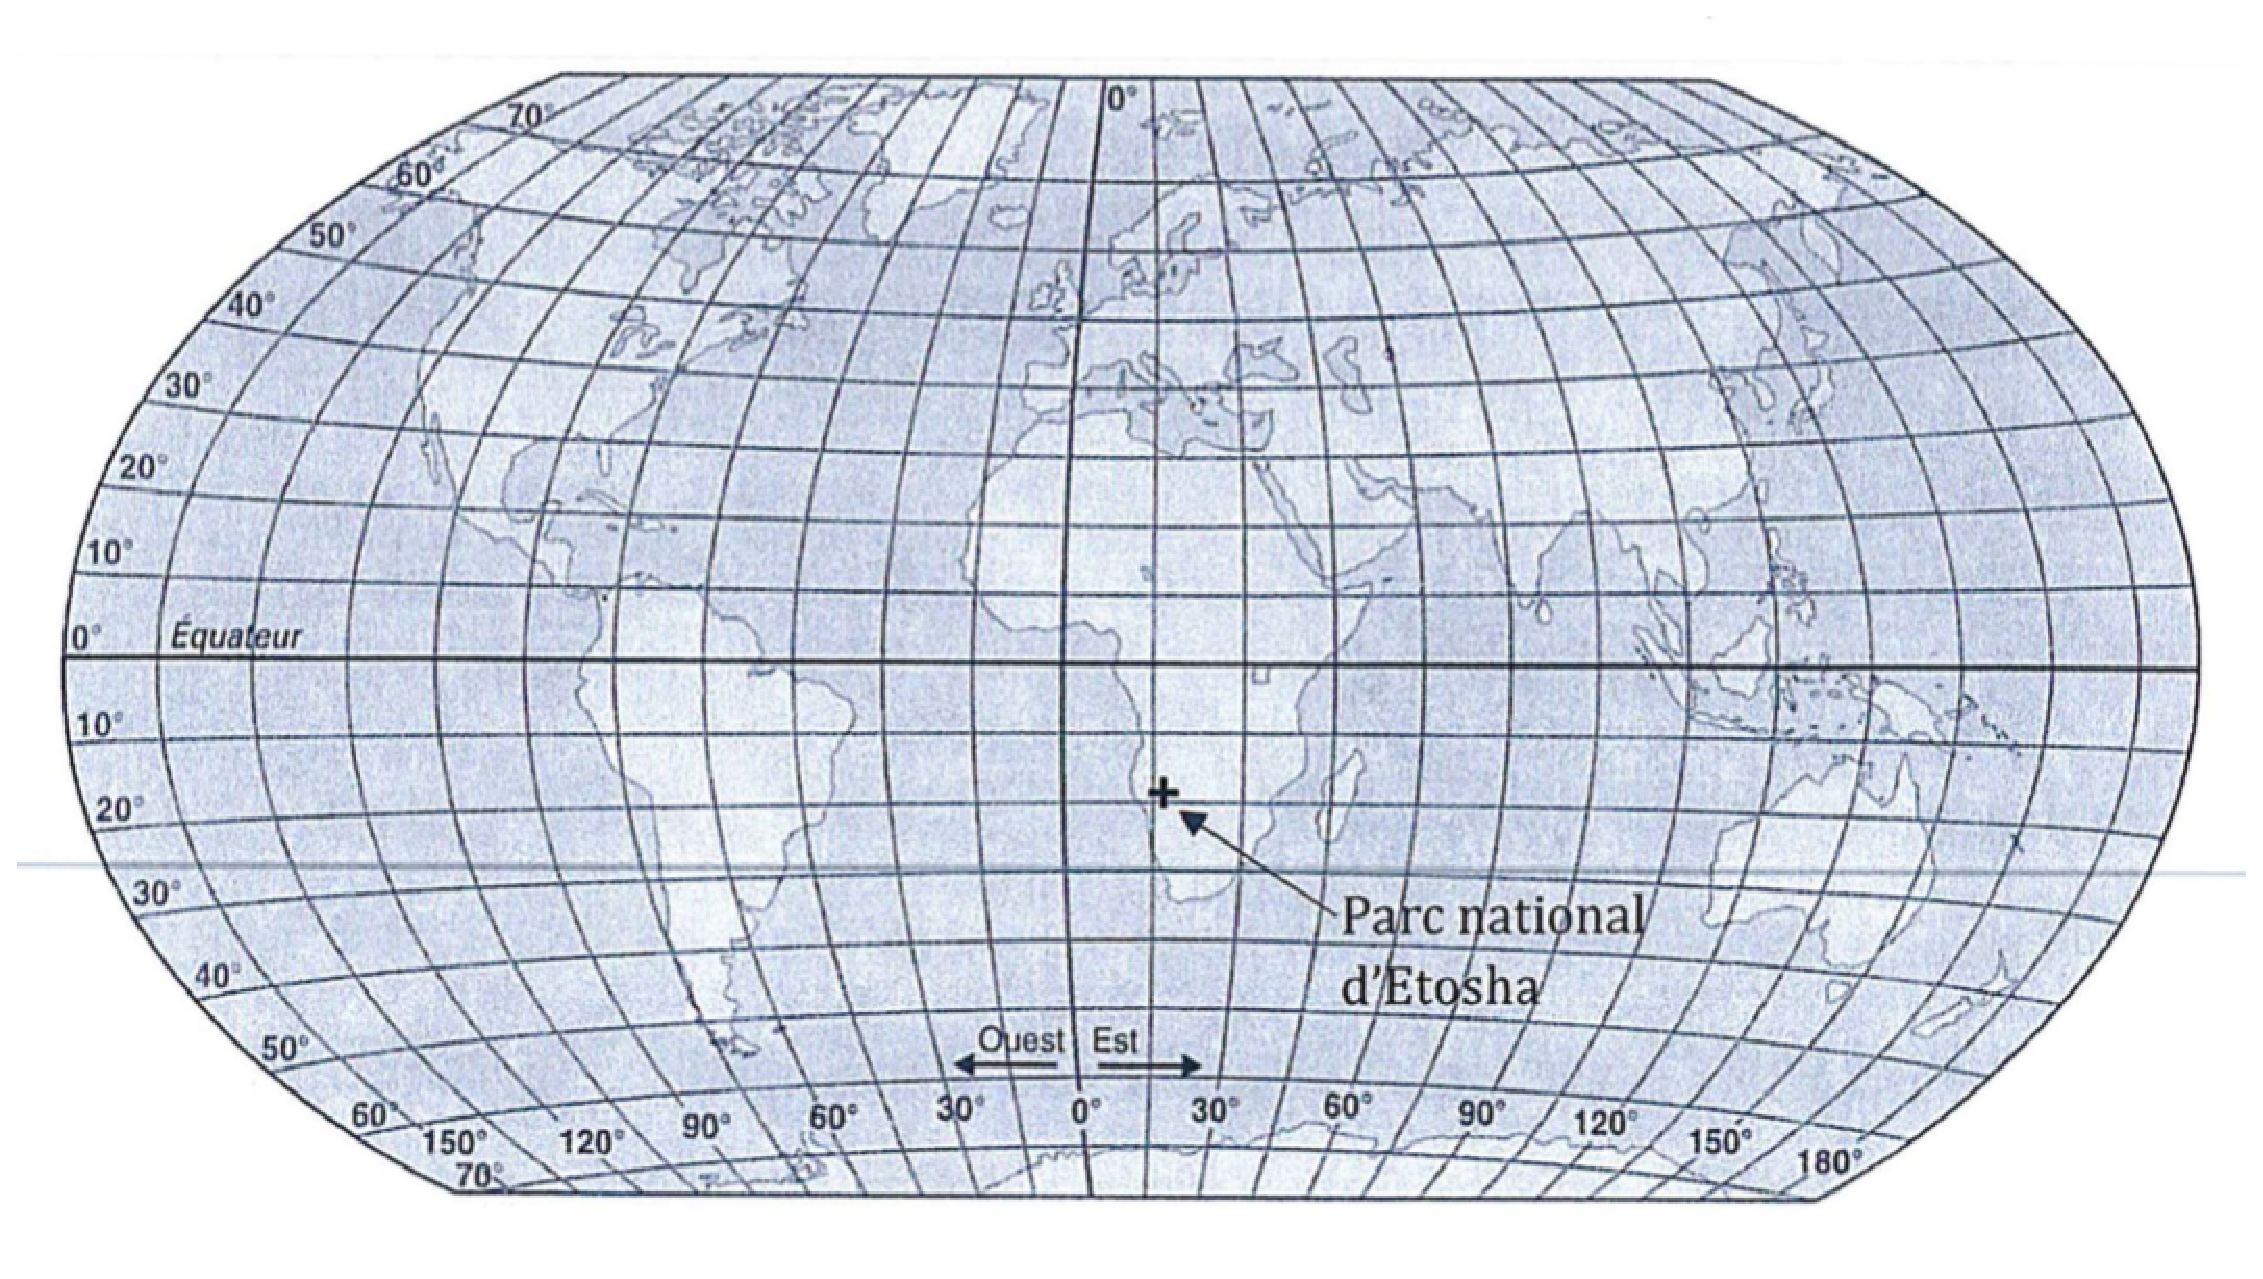
\includegraphics[width=14cm]{mappemonde.eps}

\end{enumerate}

\bigskip

\textbf{\large Exercice 4 \hfill 20 points}

\medskip

On dispose d'un terrain en pente sur lequel on souhaite construire une maison. Il faut pour cela enlever de la terre afin d'obtenir un terrain horizontal.
On dispose des informations suivantes :

\medskip

\begin{minipage}{0.28\linewidth}
La maison sera construite sur le terrain horizontal représenté par le segment [BC].
Le triangle ABC est rectangle en C et : 

AC $= 2,6$ m

AB $=17$ m
\end{minipage}\hfill
\begin{minipage}{0.67\linewidth}
\psset{unit=0.8cm}
\begin{pspicture}(12,5.5)
\pspolygon[fillstyle=dots,hatchcolor=lightgray,linecolor=white](0,0)(12,0)(12,1)(3.2,1)(3.2,2.4)(0,2.4)
\pspolygon[fillstyle=hlines,hatchcolor=gray,linecolor=white](8.3,1)(3.2,2.4)(3.2,1)%BAC
\psframe(3.2,1)(3.4,1.2)
\rput(6,2.8){Terre à enlever}\psline{->}(6,2.4)(5,1.6)
\pspolygon[fillstyle=solid,fillcolor=lightgray](0.5,2.4)(0.5,3.2)(1.4,4.6)(2.3,3.2)(2.3,2.4)
\pspolygon[fillstyle=solid,fillcolor=lightgray](9.7,1)(9.7,1.8)(10.6,3.2)(11.7,1.8)(11.7,1)
\uput[d](8.3,1){B} \uput[u](3.2,2.4){A} \uput[dl](3.2,1){C} 
\rput(6,5.3){\textbf{Vue en coupe du terrain}}
\psline(12,1)(3.2,1)(3.2,2.4)(0,2.4)
\psline[linestyle=dashed](8.3,1)(3.2,2.4)
\end{pspicture}
\end{minipage}

\medskip

\begin{enumerate}
\item Justifier que la longueur CB est égale à 16,8 m.
\item Le coût des travaux pour enlever la terre dépend de la mesure de l'angle $\widehat{\text{ABC}}$.
Si la mesure de l'angle $\widehat{\text{ABC}}$ est supérieure à $8,5\degres$, cela entraînera un surcoût des travaux (c'est-à-dire que les travaux pour enlever la terre coûteront plus cher).

Est-ce le cas pour ce terrain?
\item On admet que le volume de terre enlevée correspond au volume du prisme droit CBAFED de hauteur [CF] et de bases triangulaires ACB et DFE, comme représenté ci-dessous. On rappelle que les longueurs CF et AD sont égales.

% figure prisme de terre
\begin{center}
\psset{unit=1cm}
\begin{pspicture}(5.4,3.2)
\pspolygon(0.2,0.5)(2.5,0.2)(0.2,1.7)%CBA
\psline(2.5,0.2)(4.7,1.2)(2.4,2.7)(0.2,1.7)%BEDA
\psline[linestyle=dashed](0.2,0.5)(2.4,1.5)(4.7,1.2)%CFE
\psline[linestyle=dashed](2.4,1.5)(2.4,2.7)%FD
\uput[ul](0.2,1.7){A} \uput[dr](2.5,0.2){B} \uput[dl](0.2,0.5){C}
\uput[u](2.4,2.7){D} \uput[r](4.7,1.2){E} \uput[l](2.4,1.7){F}
\psframe(0.2,0.5)(0.4,0.7)\psframe(2.4,1.5)(2.6,1.7)
\rput{90}(-0.1,1.1){2,6 m}\rput{-30}(3.6,2.3){17 m}\rput{24}(1.2,2.5){30 m}
\end{pspicture}
\end{center}

Déterminer le volume de terre à enlever en m$^3$.

On rappelle la formule:

Volume d'un prisme droit = aire d'une base du prisme $\times$ hauteur du prisme.
\end{enumerate}

\bigskip

\textbf{\large Exercice 5 \hfill 14 points}

\bigskip

Dans cet exercice, aucune justification n'est attendue pour les réponses apportées aux questions 1. et 2.

À l'aide d'un logiciel de programmation, on définit un bloc \og Losange\fg{} pour construire un losange.

\begin{center}
\begin{tabularx}{\linewidth}{|*{2}{>{\centering \arraybackslash}X|}}\hline
\textbf{Bloc \og Losange \fg }\rule{0pt}{15pt}&\textbf{Losange obtenu}\\
&\\
\parbox{5cm}{
\begin{scratch}[pre text=\bf\sffamily,scale=0.75]
\initmoreblocks{définir \namemoreblocks{Losange}}
\blockpen{stylo en position d'écriture}
\blockrepeat{répéter \ovalnum{2} fois}
{
\blockmove{avancer de \ovalnum{20}}
\blockmove{tourner \turnright{} de \ovalnum{60} degrés}
\blockmove{avancer de \ovalnum{$a$}}
\blockmove{tourner \turnright{} de \ovalnum{$b$} degrés}
}
\blockpen{relever le stylo}
\end{scratch}
}% fin du parbox
&
\parbox{5cm}{
\psset{unit=1cm,arrowsize=2pt 3}
\begin{pspicture}(0,-5)(4.2,1.3)
\pspolygon(3.3,0.7)(4.1,0.7)(4.45,0)(3.65,0)
%\psgrid 
\psline{->}(2.6,0.7)(3.3,0.7)
\uput[r](0,1.1){Point et}
\uput[r](0,0.7){orientation de}
\uput[r](0,0.3){départ}
\end{pspicture}
}
\\ 
&\\
 \hline
\end{tabularx}
\end{center}

\medskip

\begin{enumerate}
\item Dans le bloc \og Losange \fg, par quelles valeurs faut-il remplacer $a$ et $b$ pour obtenir le losange ci-dessus ?
\item On définit ensuite un nouveau bloc nommé \og Motif A \fg{} :

\begin{center}
\begin{scratch}[pre text=\bf\sffamily,scale=0.75]
\initmoreblocks{définir \namemoreblocks{Motif A}}
\blockrepeat{répéter \ovalnum{3} fois}
{
\blockmove{Losange}
\blockmove{tourner \turnright{} de \ovalnum{60} degrés}
}
\end{scratch}
\end{center}

Parmi les figures suivantes, quelle est celle qui est obtenue en exécutant le bloc \og Motif A\fg{} ?

\begin{center}
\begin{tabularx}{\linewidth}{|*{3}{>{\centering \arraybackslash}X|}}\hline
Figure 1& Figure 2& Figure 3\\ \hline
\psset{unit=1cm}
\begin{pspicture}(-2,-2)(2,2)
\def\petale{\pspolygon(0,0)(1;0)(1.732;-30)(1;-60)}
\multido{\n=0+-45}{3}{\rput{\n}(0,0){\petale}}

\end{pspicture}&
\psset{unit=1cm}
\begin{pspicture}(-2,-2)(2,2)
\def\petale{\pspolygon(0,0)(1;0)(1.732;30)(1;60)}
\multido{\n=0+60}{6}{\rput{\n}(0,0){\petale}}
\end{pspicture}&\psset{unit=1cm}
\begin{pspicture}(-2,-2)(2,2)
\def\petale{\pspolygon(0,0)(1;0)(1.732;-30)(1;-60)}
\multido{\n=0+-60}{3}{\rput{\n}(0,0){\petale}}

\end{pspicture}\\ \hline
\end{tabularx}
\end{center}

\item On a défini un nouveau bloc nommé \og Motif B \fg. En l'exécutant, on a obtenu la figure ci-dessous:

\begin{center}
\psset{unit=1cm}
\begin{pspicture}(0,-1)(6,0.1)
%\psgrid
\def\petale{\pspolygon(0,0)(1;0)(1.732;-30)(1;-60)}
\multido{\n=0+2}{3}{\rput(\n,0){\petale}}
\end{pspicture}
\end{center}

Écrire un script du bloc \og Motif B \fg.
\end{enumerate}
%%%   fin Amérique du Sud 2 décembre 2024
\newpage
%%% Nouvelle-Calédonie décembre 2024
\phantomsection

\hypertarget{Caledoniedec}{}
\label{Caledoniedec}

Pas de sujet papier : lés élèves sont notés par contrôle continu.
\phantomsection
\hypertarget{Index}{}
\setlength{\columnsep}{1.5cm}
\printindex
\end{document}